\documentclass[xcolor=dvipsnames,aspectratio=169]{beamer}
\usepackage{tabls}
\usepackage{graphicx}
\usepackage{xcolor}
\usepackage{tikz}
\usepackage{amsmath}
\usepackage{float}
\usepackage{siunitx}
\usepackage{appendixnumberbeamer} %I think this makes it so that appendices don't count toward total pages
\usepackage{array}
\usepackage{multicol}
\usepackage{amsbsy} %For better bolding
\usepackage{bbold}
%%%%%%%%%%%%%%%%%%%
%%%%%%%%%%%%%%%%%%%

%%%%%%%%%%%%%%%%%%%%%%%%%%%%%%%%%%%%%%%%%%%%%%%%%%%%%%%%%%%%%%
%%%%%%%%%%%%%%%%%%%%%%%%%%%%%%%%%%%%%%%%%%%%%%%%%%%%%%%%%%%%%%
%%%%%%%%%%%%%%%%%%%%%%%%%%%%%%%%%%%%%%%%%%%%%%%%%%%%%%%%%%%%%%
%%%%%%%%%%%%%%%%%%%%%%%%%%%%%%%%%%%%%%%%%%%%%%%%%%%%%%%%%%%%%%
%%%%%%%%%%%%%%%%%%%%%%%%%%%%%%%%%%%%%%%%%%%%%%%%%%%%%%%%%%%%%%
%%%  Ben's customizations below
%%%%%%%%%%%%%%%%%%%%%%%%%%%%%%%%%%%%%%%%%%%%%%%%%%%%%%%%%%%%%%
%%%%%%%%%%%%%%%%%%%%%%%%%%%%%%%%%%%%%%%%%%%%%%%%%%%%%%%%%%%%%%
%%%%%%%%%%%%%%%%%%%%%%%%%%%%%%%%%%%%%%%%%%%%%%%%%%%%%%%%%%%%%%
%%%%%%%%%%%%%%%%%%%%%%%%%%%%%%%%%%%%%%%%%%%%%%%%%%%%%%%%%%%%%%
%%%%%%%%%%%%%%%%%%%%%%%%%%%%%%%%%%%%%%%%%%%%%%%%%%%%%%%%%%%%%%
\usepackage{ulem}

%Custom packages
\usepackage{nth} %Format dates
\usepackage{resizegather} % Automatically resize equations in gather to fit page
\usepackage{hyperref} % Better links
\usepackage[export]{adjustbox} %right/left-aligned figures
\usepackage[style=footnote-dw]{biblatex} %Footnote citations within slide
\usepackage{subcaption} %Subfigures
\usepackage{booktabs} % \toprule, \midrule, \bottomrule in tables
\usepackage[english]{babel} %I forgot why I have this
\usepackage{amsfonts} %I forgot why I have this
%\addbibresource{bibliography.bib}
\usepackage{physics}
\newcommand\redout{\bgroup\markoverwith
{\textcolor{red}{\rule[0.5ex]{2pt}{2pt}}}\ULon}
\renewcommand<>{\redout}[1]{
  \only#2{\beameroriginal{\redout}{#1}}
  \invisible#2{#1}
}
\bibliography{bibliography}
\newcolumntype{P}[1]{>{\centering\arraybackslash}p{#1}}

%I don't remember why I had this... I think it makes itemize look the way I wanted
\newlength{\wideitemsep}
\setlength{\wideitemsep}{8pt}
\let\olditem\item
\renewcommand{\item}{\setlength{\itemsep}{\wideitemsep}\olditem}
\usepackage{algorithm,algorithmic}
%Shortcuts to Greek letters:
\newcommand{\eps}{\epsilon}
\newcommand{\veps}{\varepsilon}
\newcommand{\g}{\gamma}
\newcommand{\w}{\omega}
\newcommand{\W}{\Omega}
\newcommand{\z}{\zeta}
% Vector symbols:
\newcommand{\bW}{\boldsymbol{\hat{\Omega}}}
\newcommand{\bWp}{\boldsymbol{\hat{\Omega}'}}
\newcommand{\br}{\boldsymbol{r}}
\newcommand{\bphi}{\pmb{\phi}}

%I'm lazy and don't want to type these out:
\renewcommand{\l}{\left}  %This one in particular might interfere with things, so be careful
\renewcommand{\r}{\right}
\newcommand{\la}{\left\langle}
\newcommand{\ra}{\right\rangle}

% Useful shortcut for referring to equations:
\newcommand{\refeqn}[1]{Equation~\eqref{eqn:#1}}
\newcommand{\refeqns}[1]{Equations~\eqref{eqns:#1}}
% The tilde prevents line breaks between the word "Equation(s)" and the eq. #

%Reduce spacing before+after equations:
\setlength{\abovedisplayskip}{0pt}
\setlength{\belowdisplayskip}{0pt}
\setlength\abovedisplayshortskip{0pt}
\setlength\belowdisplayshortskip{0pt}

% More shortcuts because I'm lazy:
\newcommand{\dx}{\Delta x}
\newcommand{\dy}{\Delta y}
\newcommand{\dz}{\Delta z}
\newcommand{\sumg}{\sum\limits_{g=1}^G}
\newcommand{\sumgp}{\sum\limits_{g'=1}^G}
\newcommand{\sumgpp}{\sum\limits_{g''=1}^G}
\newcommand{\half}{\frac{1}{2}}
    
%Underline:
\newcommand{\und}{\underline}
%Tilde:
\newcommand{\wt}{\widetilde}
%Silly hack to get the overline to be a little bit higher:
\newcommand{\ol}[1]{\overline{\vphantom{f^{{o}_f}}#1}}
\newcommand{\olf}[1]{\overline{\vphantom{f^{i}}#1}}

%Colored text shortcuts:
\newcommand{\colg}[1]{{\color{ForestGreen} #1}}
\newcommand{\colb}[1]{{\color{blue} #1}}
\newcommand{\colr}[1]{{\color{red} #1}}
\newcommand{\colo}[1]{{\color{orange} #1}}
\newcommand{\colcy}[1]{{\color{cyan} #1}}

\newcommand{\bBr}[1]{\Big[ #1 \Big]}
\newcommand{\bSr}[1]{\Big( #1 \Big)}
\newcommand{\blr}[1]{\Big| #1 \Big|}

%%%%%%%%%%%%%%%%%%%%%%%%%%%%%%%%%%%%%%%%%%%%%%%%%%%%%%%%%%%%%%
%%%%%%%%%%%%%%%%%%%%%%%%%%%%%%%%%%%%%%%%%%%%%%%%%%%%%%%%%%%%%%
%%%%%%%%%%%%%%%%%%%%%%%%%%%%%%%%%%%%%%%%%%%%%%%%%%%%%%%%%%%%%%
%%%%%%%%%%%%%%%%%%%%%%%%%%%%%%%%%%%%%%%%%%%%%%%%%%%%%%%%%%%%%%
%%%%%%%%%%%%%%%%%%%%%%%%%%%%%%%%%%%%%%%%%%%%%%%%%%%%%%%%%%%%%%
%%% More customizations (these are more beamer-specific)
%%%%%%%%%%%%%%%%%%%%%%%%%%%%%%%%%%%%%%%%%%%%%%%%%%%%%%%%%%%%%%
%%%%%%%%%%%%%%%%%%%%%%%%%%%%%%%%%%%%%%%%%%%%%%%%%%%%%%%%%%%%%%
%%%%%%%%%%%%%%%%%%%%%%%%%%%%%%%%%%%%%%%%%%%%%%%%%%%%%%%%%%%%%%
%%%%%%%%%%%%%%%%%%%%%%%%%%%%%%%%%%%%%%%%%%%%%%%%%%%%%%%%%%%%%%

%This theme is nice because it has navigation circles and looks nice:
\usetheme{Frankfurt}
\usecolortheme[RGB={0,0,153}]{structure}

%Make sure the footnote doesn't collide with the navigation symbols on the bottom of the slide:
% \addtobeamertemplate{footnote}{}{\vspace{5ex}}
%This hack doesn't work if you have more than one footnote... so in that case, you'll have to do something else

\addtobeamertemplate{footnote}{\vspace{-6pt}\advance\hsize-0.5cm}{\vspace{8pt}}
\makeatletter
% Alternative A: footnote rule
\renewcommand*{\footnoterule}{\kern -3pt \hrule \@width 2in \kern 8.6pt}
% Alternative B: no footnote rule
% \renewcommand*{\footnoterule}{\kern 6pt}
\makeatother


%Text margins:
\setbeamersize{text margin left=1em,text margin right=1em}

%Font sizes in titles:
\setbeamerfont{frametitle}{size=\large}
\setbeamerfont{normal font}{size=\tiny}

%I think this is the UM logo on the bottom left of every slide?
\pgfdeclareimage[height=0.15in]{UMlogo}{michigan_engineering2.png}
\usepackage{eso-pic}
\newcommand\AtPagemyUpperLeft[1]{\AtPageLowerLeft{%
\put(\LenToUnit{0.01\paperwidth},\LenToUnit{0.01\paperwidth}){#1}}}
\AddToShipoutPictureFG{
  \AtPagemyUpperLeft{{\pgfuseimage{UMlogo}}}
}%

% Logo for title page:
\titlegraphic{
\includegraphics[height=0.2\textheight]{michigan_block_m.png}}

\setbeamerfont{footnote}{size=\fontsize{2pt}{0pt}\selectfont}
\addtobeamertemplate{footnote}{\vspace{-1pt}\advance\hsize-0.1cm}{\vspace{1pt}}

% Frame numbers (and navigation symbols?):
\addtobeamertemplate{navigation symbols}{}{%
    \usebeamerfont{footline}%
    \usebeamercolor[fg]{footline}%
    \hspace{1em}%
    \insertframenumber/\inserttotalframenumber
}

%%%% Commands to turn navigation circles on/off:
\makeatletter
\let\beamer@writeslidentry@miniframeson=\beamer@writeslidentry
\def\beamer@writeslidentry@miniframesoff{%
  \expandafter\beamer@ifempty\expandafter{\beamer@framestartpage}{}% does not happen normally
  {%else
    % removed \addtocontents commands
    \clearpage\beamer@notesactions%
  }
}
\newcommand*{\miniframeson}{\let\beamer@writeslidentry=\beamer@writeslidentry@miniframeson}
\newcommand*{\miniframesoff}{\let\beamer@writeslidentry=\beamer@writeslidentry@miniframesoff}
\makeatother

\setbeamerfont{section in toc}{size=\normalsize}
\setbeamerfont{subsection in toc}{size=\small}

%%%% Define an environment with the margin style I want for outline slides
\newenvironment{chg}{%
   \begin{list}{}{%
      \setlength{\leftmargin}{1cm}%
   }%
\item[]}{\end{list}}

%Outline page at beginning of each section:
\AtBeginSection[]
{
    \begin{frame}<beamer>[noframenumbering] %disable increment of frame number
    \vfill
    \begin{chg}
    \begin{minipage}[c][4cm]{0.8\textwidth}
        \tableofcontents[currentsection]
    \end{minipage}
    \end{chg}
    \vfill
    \end{frame}
}

%Outline page at beginning of each subsection, other subsections greyed out:
\AtBeginSubsection[]
{
    \miniframesoff % in this miniframesoff environment, we don't get navigation circles for subsection outline slides
    \begin{frame}<beamer>[noframenumbering]
    \vfill
    \begin{chg}
    \begin{minipage}[c][4cm]{0.8\textwidth}
        \tableofcontents[sectionstyle=show/shaded, currentsubsection]
    \end{minipage}
    \end{chg}
    \vfill
    \end{frame}
    \miniframeson
}

\usepackage{tikz} %For drawing stuff
\usetikzlibrary{calc} %Coordinate calculations
\tikzset{mystyle/.style={shape=circle,fill=black,scale=0.3}}
\usetikzlibrary{arrows.meta} %For the arrows below:
\tikzset{edge/.style = {->,-{Latex[width=2mm]}}} %nice arrows
\newcommand{\tikzmark}[1]{\tikz[overlay,remember picture] \node (#1) {};}


%%%%%%%%%%%%%%%%%%%%%%%%%%%%%%%%%%%%%%%%%%%%%%%%%%%%%%%%%%%%%%
%%%%%%%%%%%%%%%%%%%%%%%%%%%%%%%%%%%%%%%%%%%%%%%%%%%%%%%%%%%%%%
%%%%%%%%%%%%%%%%%%%%%%%%%%%%%%%%%%%%%%%%%%%%%%%%%%%%%%%%%%%%%%
%%%%%%%%%%%%%%%%%%%%%%%%%%%%%%%%%%%%%%%%%%%%%%%%%%%%%%%%%%%%%%
%%%%%%%%%%%%%%%%%%%%%%%%%%%%%%%%%%%%%%%%%%%%%%%%%%%%%%%%%%%%%%
%%%%%%%%%%%%%%%%%%%%%%%%%%%%%%%%%%%%%%%%%%%%%%%%%%%%%%%%%%%%%%
%%%%%%%%%%%%%%%%%%%%%%%%%%%%%%%%%%%%%%%%%%%%%%%%%%%%%%%%%%%%%%
%%%%%%%%%%%%%%%%%%%%%%%%%%%%%%%%%%%%%%%%%%%%%%%%%%%%%%%%%%%%%%
%%%%%%%%%%%%%%%%%%%%%%%%%%%%%%%%%%%%%%%%%%%%%%%%%%%%%%%%%%%%%%
%%%%%%%%%%%%%%%%%%%%%%%%%%%%%%%%%%%%%%%%%%%%%%%%%%%%%%%%%%%%%%

%ZZZZ check for periods

%Title info:
\title{Relationship Between Relaxation and Partial Convergence of Nonlinear Diffusion  Acceleration for Problems with Feedback}
\institute[shortinst]{ Department of Nuclear Engineering and Radiological Sciences \\ University of Michigan}
\author{Qicang Shen, Nickolas Adamowicz,  Brendan Kochunas}
\date{ August \nth{28}, 2019}

\begin{document}

%Title page:
\begin{frame}
    \titlepage
\end{frame}

%Initial outline:
\begin{frame}
\frametitle{Outline}
\begin{minipage}{0.061\linewidth}
\hfill                      
\end{minipage}
\begin{minipage}[c][4cm]{0.8\textwidth}
\tableofcontents[
hideothersubsections,
sectionstyle=show,
subsectionstyle=show
]
\end{minipage}

\end{frame}

%%%%%%%%%%%%%%%%%%%%%%%%%%%%%%%%%%%%%%%%%%
%%%%%%%%%%%%%%%%%%%%%%%%%%%%%%%%%%%%%%%%%%
%%%%%%%%%%%%%%%%%%%%%%%%%%%%%%%%%%%%%%%%%%
\section{Introduction and Motivation}


\subsection{Problem of Interest}
%%%%%%%%%%%%%%%%%%%%%%%%%%%%%%%%%%%%%%%%%%%%%%%%%%%%%%%%%%%%%%%%%%%%%%%%%%%%%%%%%%%%%%%%
\begin{frame}
	\frametitle{Multigroup Neutron Transport Equation (NTE) with Feedback}
	\vspace{-2em}
	\begin{equation}
	    \begin{aligned}
             \bW \cdot \nabla\psi_g(\br, \bW ) + \Sigma_{t,g}(\br,T) \psi_g(\br, \bW ) &=\lambda \frac{\chi_g(\br)}{4\pi} \sumgp \nu \Sigma_{f,g'}(\br,T) \phi_{g'}(\br)\\[-11pt]
           &+ \sumgp \int_{4\pi}\Sigma_{s,g'\to g}(\br,\bWp\to \bW,T)  \psi_{g'}(\br,\bWp) d\W    \label{eqn:transport}
        \end{aligned}
    \end{equation}
    \vspace{-2em}
    \begin{equation}
        \int dV\sumg\int_{4\pi}\Sigma_f\kappa\psi_g d\W=P\label{eqn:normalization}
    \end{equation}
    \vspace{-2em}
    \begin{equation}
        \boldsymbol{L}(T)T(\br)=\sumg\Sigma_{f,g}(\br,T)\kappa\Phi_g(\br)\label{eqn:th}
    \end{equation}
    \vspace{-2em}
	\begin{itemize}
	\item The smallest $\lambda \equiv \frac{1}{k}$ eigenvalue, its corresponding eigenvector $\psi$, and the associated temperature distribution $T$ are desired from this set of coupled equations.
	\vspace{-0.5em}
	\item A normalization condition must be imposed to ensure a unique solution to the transport eigenvalue problem.
	\vspace{-0.5em}
	\end{itemize}
	\vfill
\end{frame}
%%%%%%%%%%%%%%%%%%%%%%%%%%%%%%%%%%%%%%%%%%%%%%%%%%%%%%%%%%%
\begin{frame}
\frametitle{Overall Iteration Schemes}

\vspace{-0.5em}
\begin{itemize}
    \item Iteration Scheme:
    \begin{itemize}
        \item \textbf{Picard}
        \vspace{-0.5em}
        \item Each Physics is solved separately
        \vspace{-0.5em}
        \item Easy to implement
    \end{itemize}
    \vspace{-0.2em}
    \item Transport iteration Scheme:
     \begin{itemize}
         \item Source Iteration
         \vspace{-0.5em}
         \item Iterates on eigenvalue, and scattering \\
         and fission sources
         \vspace{-0.5em}
         \item Converges very slow
     \end{itemize}
     \vspace{-0.2em}
    \item Acceleration Scheme:
    \begin{itemize}
        \item \textbf{Nonlinear Diffusion Acceleration (NDA)}
        \vspace{-0.5em}
        \item Reduce the total outer iteration number by orders of magnitude
    \end{itemize}
    \vspace{-0.2em}
    \item Eigenvalue Solver:
    \begin{itemize}
        \item Wielandt Shifted Power Iteration
    \end{itemize}
\end{itemize}
  \begin{picture}(5,5)
     \put(230,70){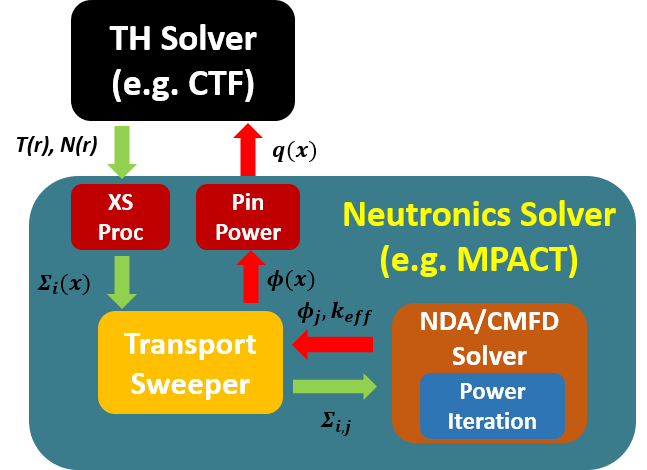
\includegraphics[width=0.45\textwidth]{Texfile/Figure/Picard.png}}
  \end{picture}
\end{frame}
%%%%%%%%%%%%%%%%%%%%%%%%%%%%%%%%%%%%%%%%%%%%%%%%%%%%%%%%%%%%%%%%%%%%%%%%%%%%%%%%%%%%%%%%%%%%%%
\begin{frame}
    \frametitle{Nonlinear Diffusion Acceleration, Coarse Mesh Finite Difference}
    \begin{itemize}
        \item Nonlinear Diffusion Acceleration (NDA) is a common acceleration method employed by the nuclear reactor community:
            \begin{itemize}
                \item Low-order, transport-corrected diffusion equation
                \vspace{-0.5em}
                \item Nonlinear correction term $\hat{D}$ obtained from a high-order transport sweep
                \vspace{-0.5em}
			    \item Scalar flux and eigenvalue solution used as an improved estimate for the scattering and fission source terms in a subsequent transport sweep
            \end{itemize}
    \end{itemize}
    \vspace{-0.25cm}
	\begin{equation}
	  \begin{aligned}
	    &\l[-\nabla \cdot D_g(\br,T) \nabla + \Sigma_{t,g}(\br,T)+\hat{D}_g(\br,T) \r] \phi_g(\br) =\\[-13pt]
	    &\hspace{4cm}\sumgp \Sigma_{s0,g' \to g} (\br,T) \phi_{g'}(\br) + \lambda \chi_g(\br) \sumgp \nu \Sigma_{f,g'}(\br,T) \phi_{g'}(\br) \end{aligned}\label{eqn:eig}
	\end{equation}\\[-1em]
	\begin{itemize}
	    \item Coarse Mesh Finite Difference (CMFD) : a generalization of NDA which allows for a coarser mesh to be used on the low-order problem
	\end{itemize}	
\end{frame}
%%%%%%%%%%%%%%%%%%%%%%%%%%%%%%%%%%%%%%%%%%%%%%%%%%%%%%%%%%%%%%%%%%%%%%%%%%%%%%%%%%%%%%%%
\begin{frame}
	\frametitle{ Wielandt-Shifted Power Iteration}
	\begin{itemize}
	    \item Martix form of \refeqn{eig}:
	    \begin{equation}
	        \mathbf{M\phi}=\lambda\mathbf{F}\phi
	    \end{equation}
	    \vspace{-1.5em}
		\item Standard power iteration (PI):
				\begin{gather}
					\mathbf{M} {\bphi}^{(l+1)} = \lambda^{(l)} \mathbf{F}  \bphi^{(l)}  \\
					\lambda^{(l+1)} = \lambda^{(l)} \| \mathbf{F} \bphi^{(l)}\|/\| \mathbf{F} \bphi^{(l+1)}\|
				\end{gather}
		PI converges at a rate equal to the dominance ratio (DR): $\lambda_1/\lambda_2$
		\vspace{-0.3em}
		\item Because the DR is close to 1 for realistic reactor problems, we can improve the spectral radius of PI using a Wielandt Shift (WS):
			\begin{equation}
				\l[ \mathbf{M} - \lambda_s\mathbf{F} \r] \bphi^{(l+1)} = \l[ \lambda^{(l)} - \lambda_s \r] \mathbf{F}  \bphi^{(l)} \label{eqn:WS}
			\end{equation}
		\item In practice, this ``inner'' iteration procedure is not full converged, instead it is truncated at a given total number of iterations $L$ or when some other convergence criteria is met
	\end{itemize}
\end{frame}

\subsection{Motivation}
%%%%%%%%%%%%%%%%%%%%%%%%%%%%%%%%%%%%%%%%%%%%%%%%%%%%%%%%%%%%%%%%%%%%%%%%%%%%%%%%%%%%%%%%
\begin{frame}
\vspace{-1.5em}
\frametitle{Picard iteration scheme is more stable than we have expected}
\tikzmark{mybox}{}
\begin{itemize}
\item Drawbacks of the Picard scheme:\\[0.2em]
\begin{itemize}
    \item Stability is not guaranteed
    \vspace{-0.5em}
    \item Relaxation is always used
\end{itemize}
\vspace{-0.5em}
\item Furthermore, Theoretical Analysis~\footfullcite{Kochunas2017FourierSections}:\\[0.2em]
\begin{itemize}
    \item Relaxation could not help \\
    when $\Sigma_tX>100$
    \vspace{-0.5em}
    \item Hmm, the optical thickness of a 3D \\
    pincell is around 100.
\end{itemize}
\vspace{2em}
\item But, the multiphysics simulations have been performed for full core problems\\[0.2em].

\end{itemize}
    \begin{picture}(5,5)
     \put(220,35){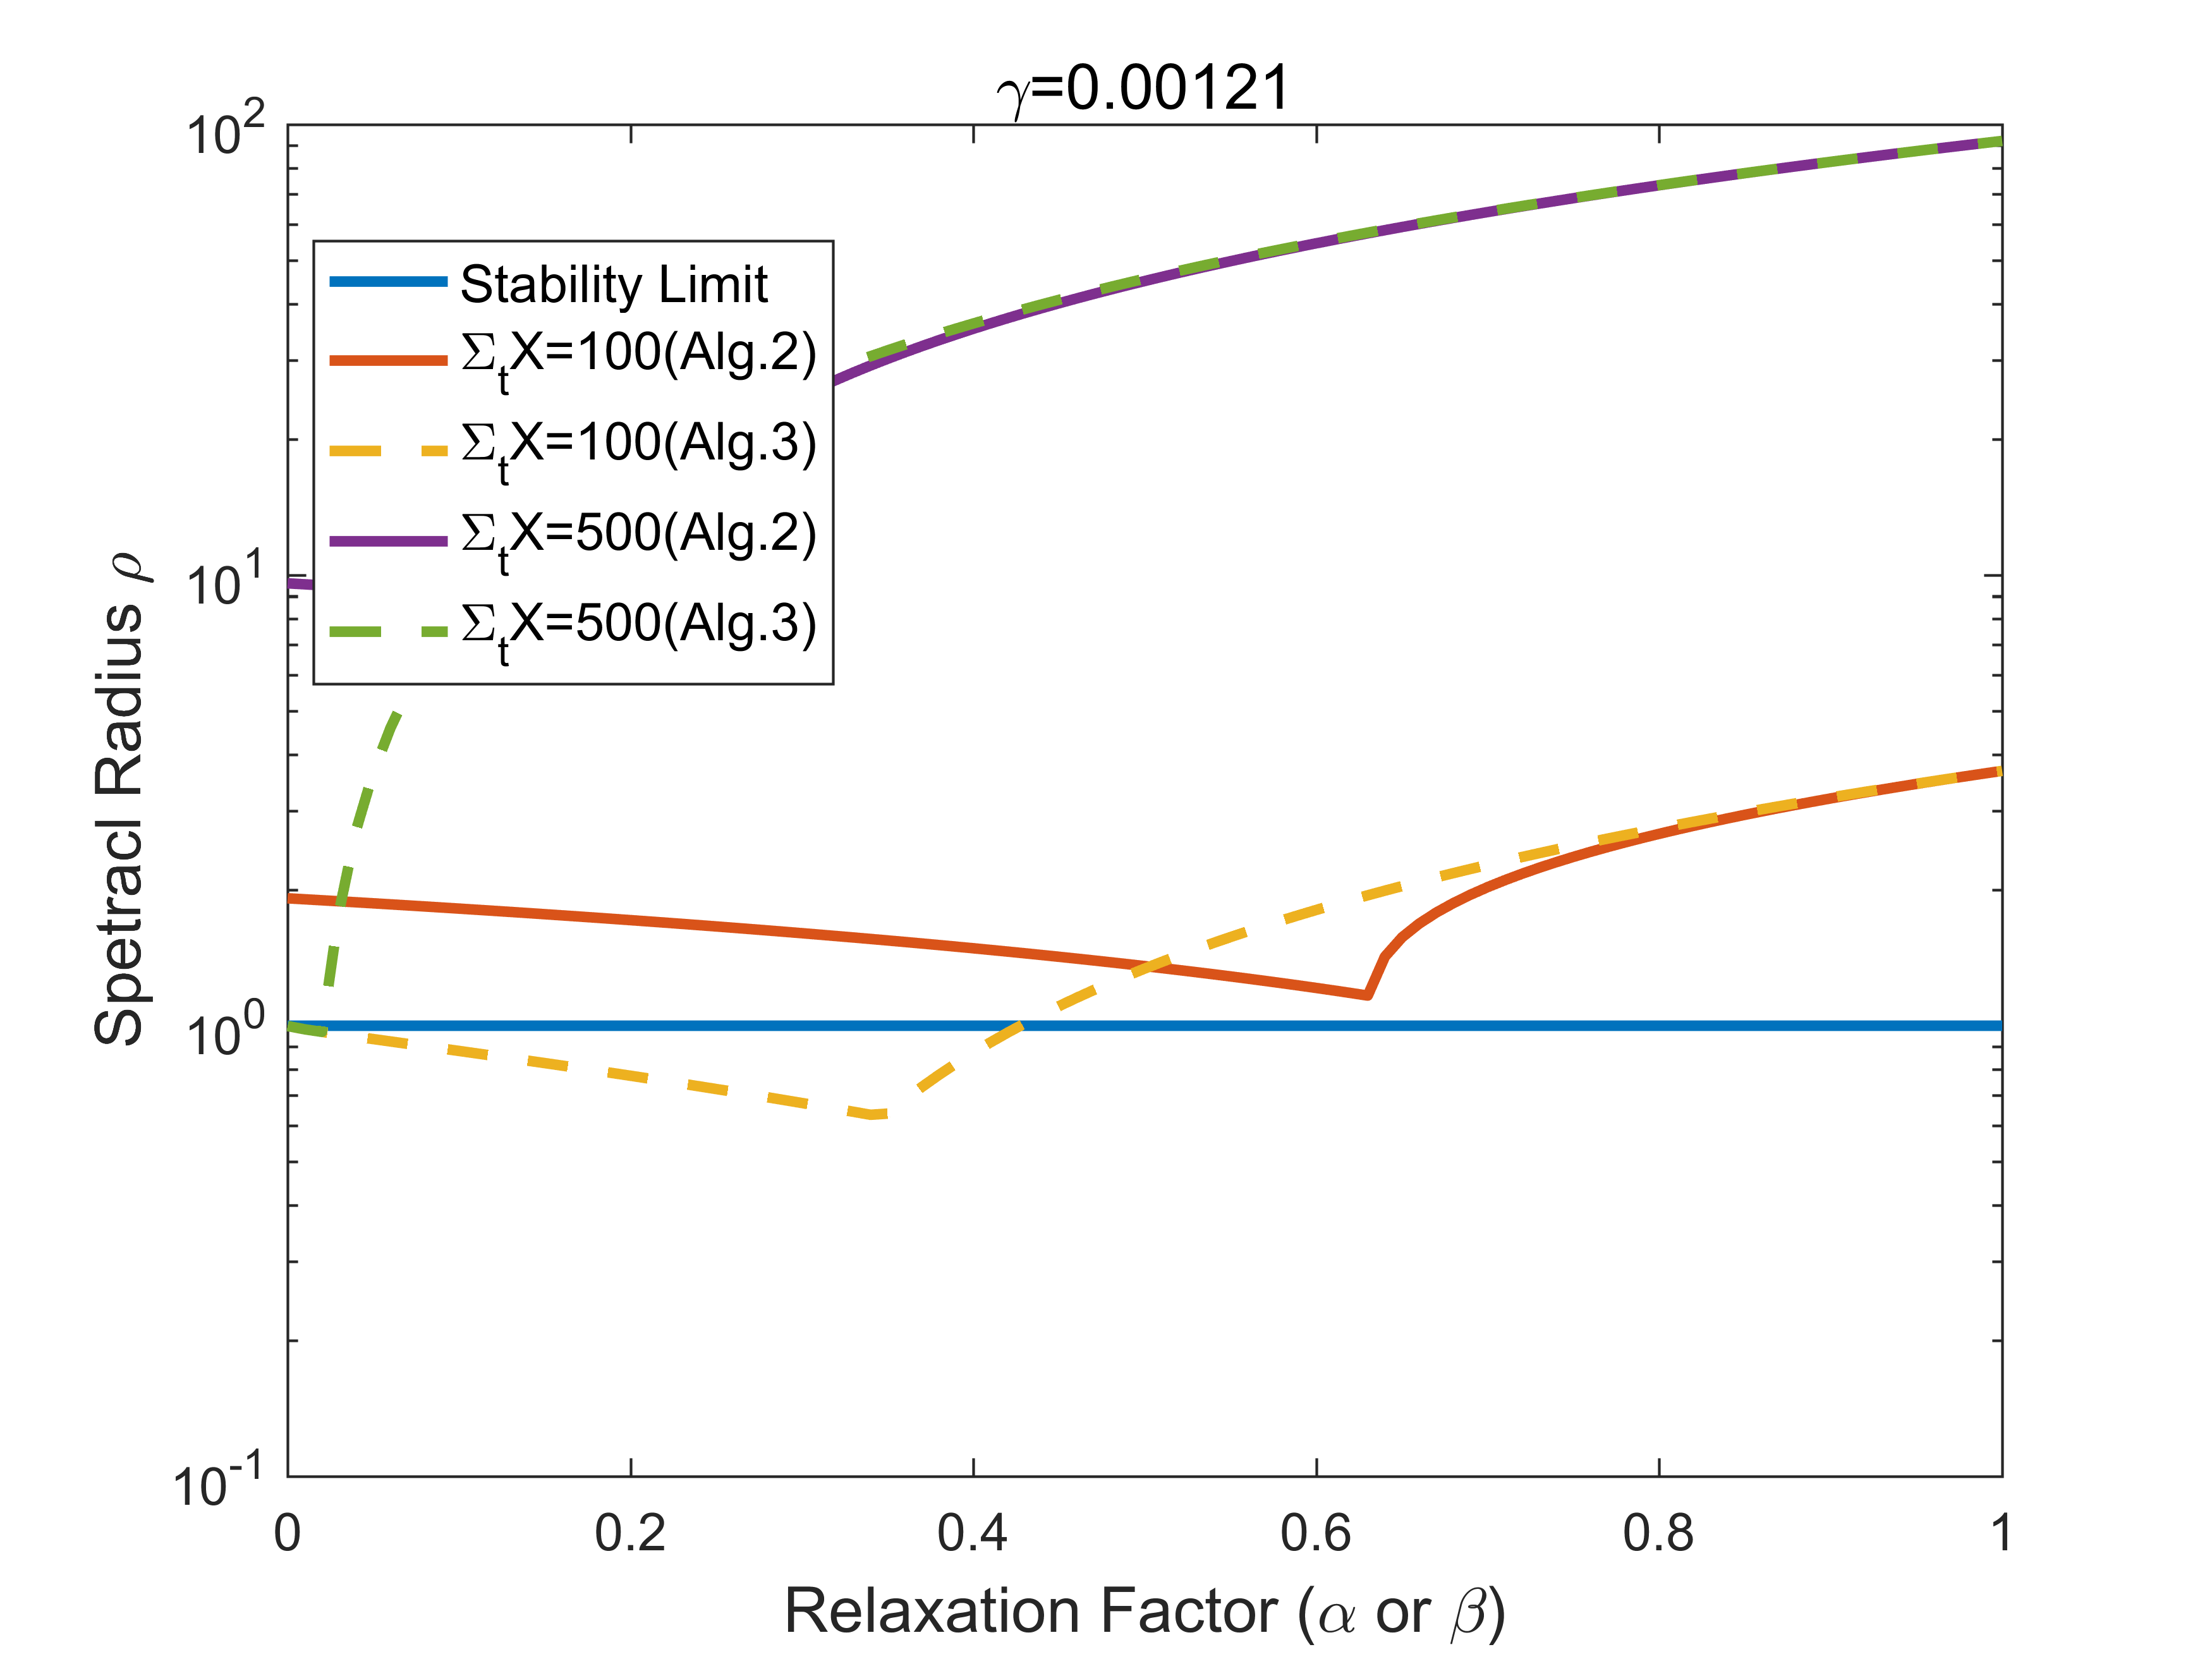
\includegraphics[width=0.45\textwidth]{Texfile/Figure/rhovalpha_old.png}}
  \end{picture}
%   \tikz[overlay,remember picture]{\draw[draw=red,thick,fill opacity=0] ($(mybox)+(1,-1)$) rectangle ($(mybox)+(8,-3.5)$);}
\vspace{-0.5em}
 \end{frame}


%%%%%%%%%%%%%%%%%%%%%%%%%%%%%%%%%%%%%%%%%%%%%%%%%%%%%%%%%%%%%%%%%%%%%%%%%%%%%%%%%%%%%%%%
\begin{frame} \frametitle{More accurate CMFD solutions make iterations scheme unstable}
\begin{enumerate}
    \item Example 1--3D Pin Cell
    \begin{itemize}
        \item Length: 380 $cm$, Power: 71 $kW$
        \vspace{-0.5em}
        \item $L$: $\#$ of power iteration, $nOuter$: $\#$ of total outer iteration
    \end{itemize}
    \begin{table} [!hbt]
    \centering
     \small
    \begin{tabular}{c|c|c|c|c|c|c|c|c} 
        \toprule
        \textbf{$L$}&2 & 4 & 6 & 10 & 15 & 20 &30&100\\ 
         \toprule
       \textbf{nOuter}&33&19&15&14&14&17&21&\textbf{N/A}\\
        \toprule
    \end{tabular}
    \end{table}
    \vspace{-1em}
    \item Example 2--Vera Problem 7
    \begin{table}[ht!]
        \centering
	\begin{tabular}{ccc}
    \toprule
        Method & nOuter & Total Runtime [s]  \\
        \midrule
   			Default & 15 &  10230 \\
  			MSED~\footfullcite{yee2019multilevel} & 20 &  9749 \\
  			MSED-L&  12  & 6057 \\
        \bottomrule
    \end{tabular}
    \begin{itemize}
        \item MSED-L:  A partially converged low order MSED solve with looser convergence criteria and less aggressive Wielandt shift
    \end{itemize}
\end{table}  
\end{enumerate}
\end{frame}
%%%%%%%%%%%%%%%%%%%%%%%%
%%%%%%%%%%%%%%%%%%%%%%%%%%%%%%%%%%%%%%%%%%%%%%%%%%%%%%%%%%%%%%%%%%%%%%%%%%%%%%%%%%%%%%%%%%
\begin{frame}{Goal of Research }
\vspace{-1em}
\begin{itemize}
\item \textbf{Questions to be answered}:
\begin{itemize}
    \item Can the effect of convergence of NDA (CMFD) be theoretically investigated?
    \begin{itemize}
        \item Previous researches on the stability of transport method always assume that NDA (CMFD) is fully converged.
    \end{itemize}
    \vspace{-0.5em}
    \item What is the relation between partial convergence and well-known relaxation?
        \begin{itemize}
            \item Effect of partial convergence is similar with the effect of relaxation
        \end{itemize}
    \item Whether the formula to determine near-optimal partial convergence can be derived?
        \begin{itemize}
            \item An near-optimal partial convergence seems to exist
            \vspace{-0.5em}
            \item Reduce the computational intensity-- \it{``why waste effort converging the low order problem with the wrong coefficients``}
            \vspace{-0.5em}
            \item Stabilize the iteration scheme
        \end{itemize}
\end{itemize}
\item Investigation Approach: \textbf{Fourier Analysis}
\end{itemize}
\vfill
\end{frame}

\section{Fourier Analysis}
\subsection{Analysis Overview}
\begin{frame}
	\frametitle{Fourier analysis is a technique that estimates the convergence properties of a method by looking at how error modes decay in a model problem*}
	\begin{itemize}
		\item Procedure for Fourier analysis:
		\begin{itemize}
		    \item Define 1-D homogeneous problem with reflective boundary conditions
			\item Define a ``Fourier ansatz'' consisting of equations of the form
				\begin{equation}
					\phi^{(l)}(x) = \phi_{0} + \epsilon\sum_{\omega_j} \theta(\w)^l  e^{i \w_j x} \,,
				\end{equation}
        		where $\phi_{0}$ is the exact solution and the second term is a ``small'' error of frequency $\w_j$
			\item Substitute temporary solutions of the equations  which define your method by Fourier ansatz , drop terms of $O(\eps^2)$ or smaller, and perform some algebra to obtain an eigenvalue problem for the decay rate $\theta(\w)$
			\item The spectral radius of the method is then given by $\rho = \max\limits_{\w_j}|\theta|$, $\rho<1$ -- the scheme is stable.
		\end{itemize}%
	\end{itemize}
\end{frame}
\subsection{Model Problem}
%%%%%%%%%%%%%%%%%%%%%%%%%%%%%%%%%%%%%%%%%%%%%%%%%%%%%%%%%%%%%%%%%%%%%%%%%%%%%%%%%%%%%%%%%%%%%%%%%%%%%%%%%%%
\begin{frame}
\frametitle{Model Specification}
\begin{itemize}
\item Cross section is assumed to be linearly dependent with the localized flux~\footfullcite{kastenberg1969stability}:
\begin{equation}
\Sigma_{i}^{\left(n\right)}\left(x\right) = \Sigma_{i,0} + \Sigma_{i,1} \left(\phi^{\left( n\right)}\left(x\right) - \Phi_0 \right)\label{eqn:updatexs}
\end{equation}
\vspace{-1em}
\begin{itemize}
    \item In general the relation between cross section and the flux is not this simple. However, when the solution is close to the true solution, this approximation is reasonable.
    \vspace{-0.5em}
    \item Former research~\footfullcite{Kochunas2017FourierSections} shows this assumption can make Fourier analysis tractable and reveal the stability of the Picard scheme in neutron transport calculation with feedback. 
    \item A proxy multiphysics application which maintains some representative behavior while allowing for a spatially flat solution
\end{itemize}

\end{itemize}
\vfill
\end{frame}

%%%%%%%%%%%%%%%%%%%%%%%%%%%%%%%%%%%%%%%%%%%%%%%%%%%%%%%%%%%%%%%%%%%%%%%%%%%%%%%%%%%%%%%%%%%%%%%%%%%%%%%%%
\begin{frame}{Model Iteration Scheme}

\begin{algorithm}[H]
\begin{algorithmic}[1]
\STATE{Initialize $\phi(x)$ and $J(x)$}
\FOR{$n=0$ to $N$}
\vspace{-0.2em}
\STATE{Update the Cross Section by \refeqn{updatexs}}
\vspace{-0.5em}
\STATE{Calculate the CMFD coefficients and nonlinear coupling term $\hat{D}$}
\vspace{-0.5em}
\STATE{Use the CMFD coefficients to form $M$ and $F$}
\vspace{-0.5em}
\FOR{$l=0$ to $L$}
\vspace{-0.2em}
\STATE{Solve $\l[ M - \lambda_sF \r] \bphi^{(l+1)} = \l[ \lambda^{(l)} - \lambda_s \r] F  \bphi^{(l)}$}
\vspace{-0.5em}
\ENDFOR
\vspace{-0.5em}
\STATE{Update the source of transport equation with coarse mesh solutions}
\vspace{-0.5em}
\STATE{Perform transport sweep}
\vspace{-0.5em}
\ENDFOR
\end{algorithmic}
\caption{Model Iteration Scheme}
\label{alg:seq}
\end{algorithm}
\end{frame}    

%%%%%%%%%%%%%%%%%%%%%%%%%%%%%%%%%%%%%%%%%%%%%%%%%%%%%%%%%%%%%%%%%%%%%%%%%%%%%%%%%%%%%%%%%%%%%%%%%%%%%%%%%%
 %ZZZZ emphasize importance of this analysis



\section{Analysis Results}
\subsection{Final Expression and Validation}
\begin{frame}{Important Parameters Revealed by Fourier Analysis}
\vspace{-1em}
\begin{itemize}
    \item Definition and Range
    \begin{table} [!hbt]
    \centering
     \small
    \begin{tabular}{c| P{2cm}|P{2cm}|P{2cm}|P{2cm}} 
        \toprule
         \textbf{Symbol}&c & $\gamma$ & $r$ & $\Sigma_tX$\\ 
        \midrule
       \textbf{Definition}&Scattering Ratio & Feedback intensity & Wielandt shift ratio & Problem Size (mfp)\\
        \midrule
        \textbf{Range}&$<0.96$ & $0-0.00121$ & $0.66-0.99$& $<500$\\ 
        \toprule
    \end{tabular}
    \end{table}
    \item Mathematical Expression:
\end{itemize}
% \begin{multicols}{4}
%   \begin{equation}
%     c=\frac{\Sigma_{s,0}}{\Sigma_{t,0}}
%   \end{equation}\break
%   \begin{equation}
%     \gamma_0= \left(\frac{\Sigma_{a,1}}{\Sigma_{a,0}} - \frac{ \Sigma_{f,1}}{\Sigma_{f,0}}\right) \Phi_0
%   \end{equation}\break\\
%   \begin{equation}
%   \frac{d\lambda}{d\phi}\frac{\nu\Sigma_{f,0}}{{\Sigma_{t,0}}}\label{eq:gamma_def}
%   \end{equation}
%   \begin{equation}
% r=\frac{\lambda_s}{\lambda}
%   \end{equation}
% \end{multicols}
\vspace{-1em}
\begin{subequations}
\noindent\begin{minipage}{.45\linewidth}
\centering
\begin{equation}
  c=\frac{\Sigma_{s,0}}{\Sigma_{t,0}}
\end{equation}
\end{minipage}%
\begin{minipage}{.45\linewidth}
\centering
\begin{equation}
  \gamma_0= \left(\frac{\Sigma_{a,1}}{\Sigma_{a,0}} - \frac{ \Sigma_{f,1}}{\Sigma_{f,0}}\right) \Phi_0
\end{equation}
\end{minipage}\\
\vspace{-1em}
\noindent\begin{minipage}{.45\linewidth}
\centering
\begin{equation}
  \gamma=(1-c)\gamma_0=\frac{d\lambda}{d\phi}\frac{\nu\Sigma_{f,0}}{{\Sigma_{t,0}}}
\end{equation}
\end{minipage}%
\begin{minipage}{.45\linewidth}
\centering
\begin{equation}
  r=\frac{\lambda_s}{\lambda}
\end{equation}
\end{minipage}
\end{subequations}

\vfill
\end{frame}

%%%%%%%%%%%%%%%%%%%%%%%%%%%%%%%%%%%%%%%%%%%%%%%%%%%%%%%%%%%%%%%%%%%%%%%%%%%%%%%%%%%%%%%%%%%%%%%%%%%%%%%%%%%%%%%%%%%%%%%%%%%%%%%%%
\begin{frame}{Fourier Analysis Result Expression}
\begin{itemize}
\vspace{-0.5em}
    \item Final Expression:
    \begin{align}\label{eqns:four-theta}
     \theta(\omega)=
        \begin{cases}
        \bSr{\Lambda^L-\gamma}f_{TS}(\omega)
        +\bSr{1-\Lambda^L(\omega)}\bBr{f_{NDA}(\omega)-\frac{3\gamma}{\omega^2}f_{TS}(\omega)} \;, &\text{continuous problem}\\
            \max \blr{eig\bSr{\mathbf{T}(\omega)}}\;, \text{discretized problem}
        \end{cases}
\end{align}
    where:
\vspace{-1em}
    \begin{align}
   \mathbf{T}(\omega)=\tilde{\mathbf{H}}(\omega)(1-\gamma)-\bSr{1&-\Lambda^L(\omega)}\mathbf{1}\frac{3\Sigma_t\Delta(e^{i\Sigma_t\Delta\omega}-1)\tilde{\mathbf{G}}+\gamma3(\Sigma_t\Delta)^2\frac{\mathbf{1}^T}{q}\tilde{\mathbf{H}}}{2-2cos(\Sigma_t\Delta\omega)}  \label{eq:eror_tr_mtx} \;, \\
    \tilde{\mathbf{H}}&\in\mathbb{C}^{q \times q}\;, \;\; \tilde{\mathbf{G}}\in\mathbb{C}^{1 \times q}\; ,\;\; {\mathbf{1}}\in\mathbb{C}^q\;.
    \end{align}
\item $q$: \# of fine cell per coarse mesh
\item $\tilde{\mathbf{H}},\tilde{\mathbf{G}}$~\footfullcite{Zhu2016b}: Error transition matrix in the transport sweep and current calculation.
\end{itemize}
\end{frame}
%%%%%%%%%%%%%%%%%%%%%%%%%%%%%%%%%%%%%%%%%%%%%%%%%%%%%%%%%%%%%%%%%%%%%%%%%%%%%%%%%%%%%%%%%%%%%%%%%%%%%%%%%%%%%%%%%%%%%%%%%%%%%%%%%
\begin{frame}{Fourier Analysis Result Expression}
\begin{subequations}
\small
\noindent\begin{minipage}{.3\linewidth}
\centering
\begin{equation}
 f_{TS}(\omega)=\frac{arctan(\omega)}{\omega}
\end{equation}
\end{minipage}%
\begin{minipage}{.6\linewidth}
\centering
\begin{equation}
f_{NDA}(\omega)=(1+\frac{1}{g(\omega)})f_{TS}(\omega)-\frac{1}{g(\omega)}
\end{equation}
\end{minipage}\\
\vspace{-1em}
\noindent\begin{minipage}{.3\linewidth}
\centering
\begin{equation}
  \hat{c}=1-(1-r)(1-c)
\end{equation}
\end{minipage}%
\begin{minipage}{.6\linewidth}
\centering
\begin{equation}
   \Lambda(\omega) = \frac{1 - \tilde{c}}{1 - \tilde{c} + g(\omega)}
\end{equation}
\end{minipage} \\
\vspace{-1em}
\centering
\begin{equation}
 g(\omega)=
        \begin{cases}
          \frac{1}{3}\omega^2 &\text{continuous problem} \\
          \frac{2-2cos\bSr{\Sigma_t\Delta\omega}}{3\bSr{\Sigma_t\Delta}^2}\;, &\text{discretized problem}
          \end{cases}\nonumber
\end{equation}

\vspace{-1em}
\begin{itemize}
\item $f_{TS}$: error decay rate for the pure transport source iteration
\vspace{-0.65em}
\item $f_{NDA}$: error decay rate for the NDA in problem without feedback
\vspace{-0.6em}
\item $\hat{c}$: effective scattering ratio
\vspace{-0.6em}
\item $\Lambda$: Error reduction rate per power iteration
\vspace{-0.6em}
\item $g(\omega)$: Coefficient induced by diffusion aproximation
\end{itemize}
\end{subequations}
\end{frame}

%%%%%%%%%%%%%%%%%%%%%%%%%%%%%%%%%%%%%%%%%%%%%%%%%%%%%%%%%%%%%%%%%%%%%%%%%%%%%%%%%%%%%
\begin{frame}{Validation of Fourier Analysis Results--Limitiation Check}
\vspace{-1em}
\begin{itemize}
    \item Continuous Case:
\begin{enumerate}
    \item For the case $L\rightarrow\infty$,$\gamma=0$, simplied as the expression for NDA:
    \begin{equation}
         \theta(\omega)=(1+\frac{3}{\omega^2})f_{TS}(\omega)-\frac{3}{\omega^2}
    \end{equation}
    \item For the case $L\rightarrow\infty$,$\gamma\neq0$, simplified as the expression~\footfullcite{Kochunas2017FourierSections} :
    \begin{equation}
         \theta(\omega)=f_{NDA}(\omega)-\gamma(1+\frac{3}{\omega^2})f_{TS}(\omega)
    \end{equation}
\end{enumerate} 
\item Discretized Case, $L\rightarrow\infty$,$\gamma=0$, simplied as the expression~\footfullcite{Zhu2016b}:
\begin{equation}
    \mathbf{T}(\omega)=\tilde{\mathbf{H}}(\omega)-\mathbf{1}\frac{3\Sigma_t\Delta(e^{i\Sigma_t\Delta\omega}-1)\tilde{\mathbf{G}}}{2-2cos(\Sigma_t\Delta\omega)},
\end{equation}
\end{itemize}

\end{frame}

%%%%%%%%%%%%%%%%%%%%%%%%%%%%%%%%%%%%%%%%%%%%%%%%%%%%%%%%%%%%%%%%%%%%%%%%%%%%%%%%%%%%%
\begin{frame}{Validation of Fourier Analysis Results--Comparision with Numerical Estimation}
\vspace{-2em}
 \begin{figure}
	\centering
	\captionsetup[subfigure]{justification=centering}
	\begin{subfigure}[t]{0.4\textwidth}
		\centering
		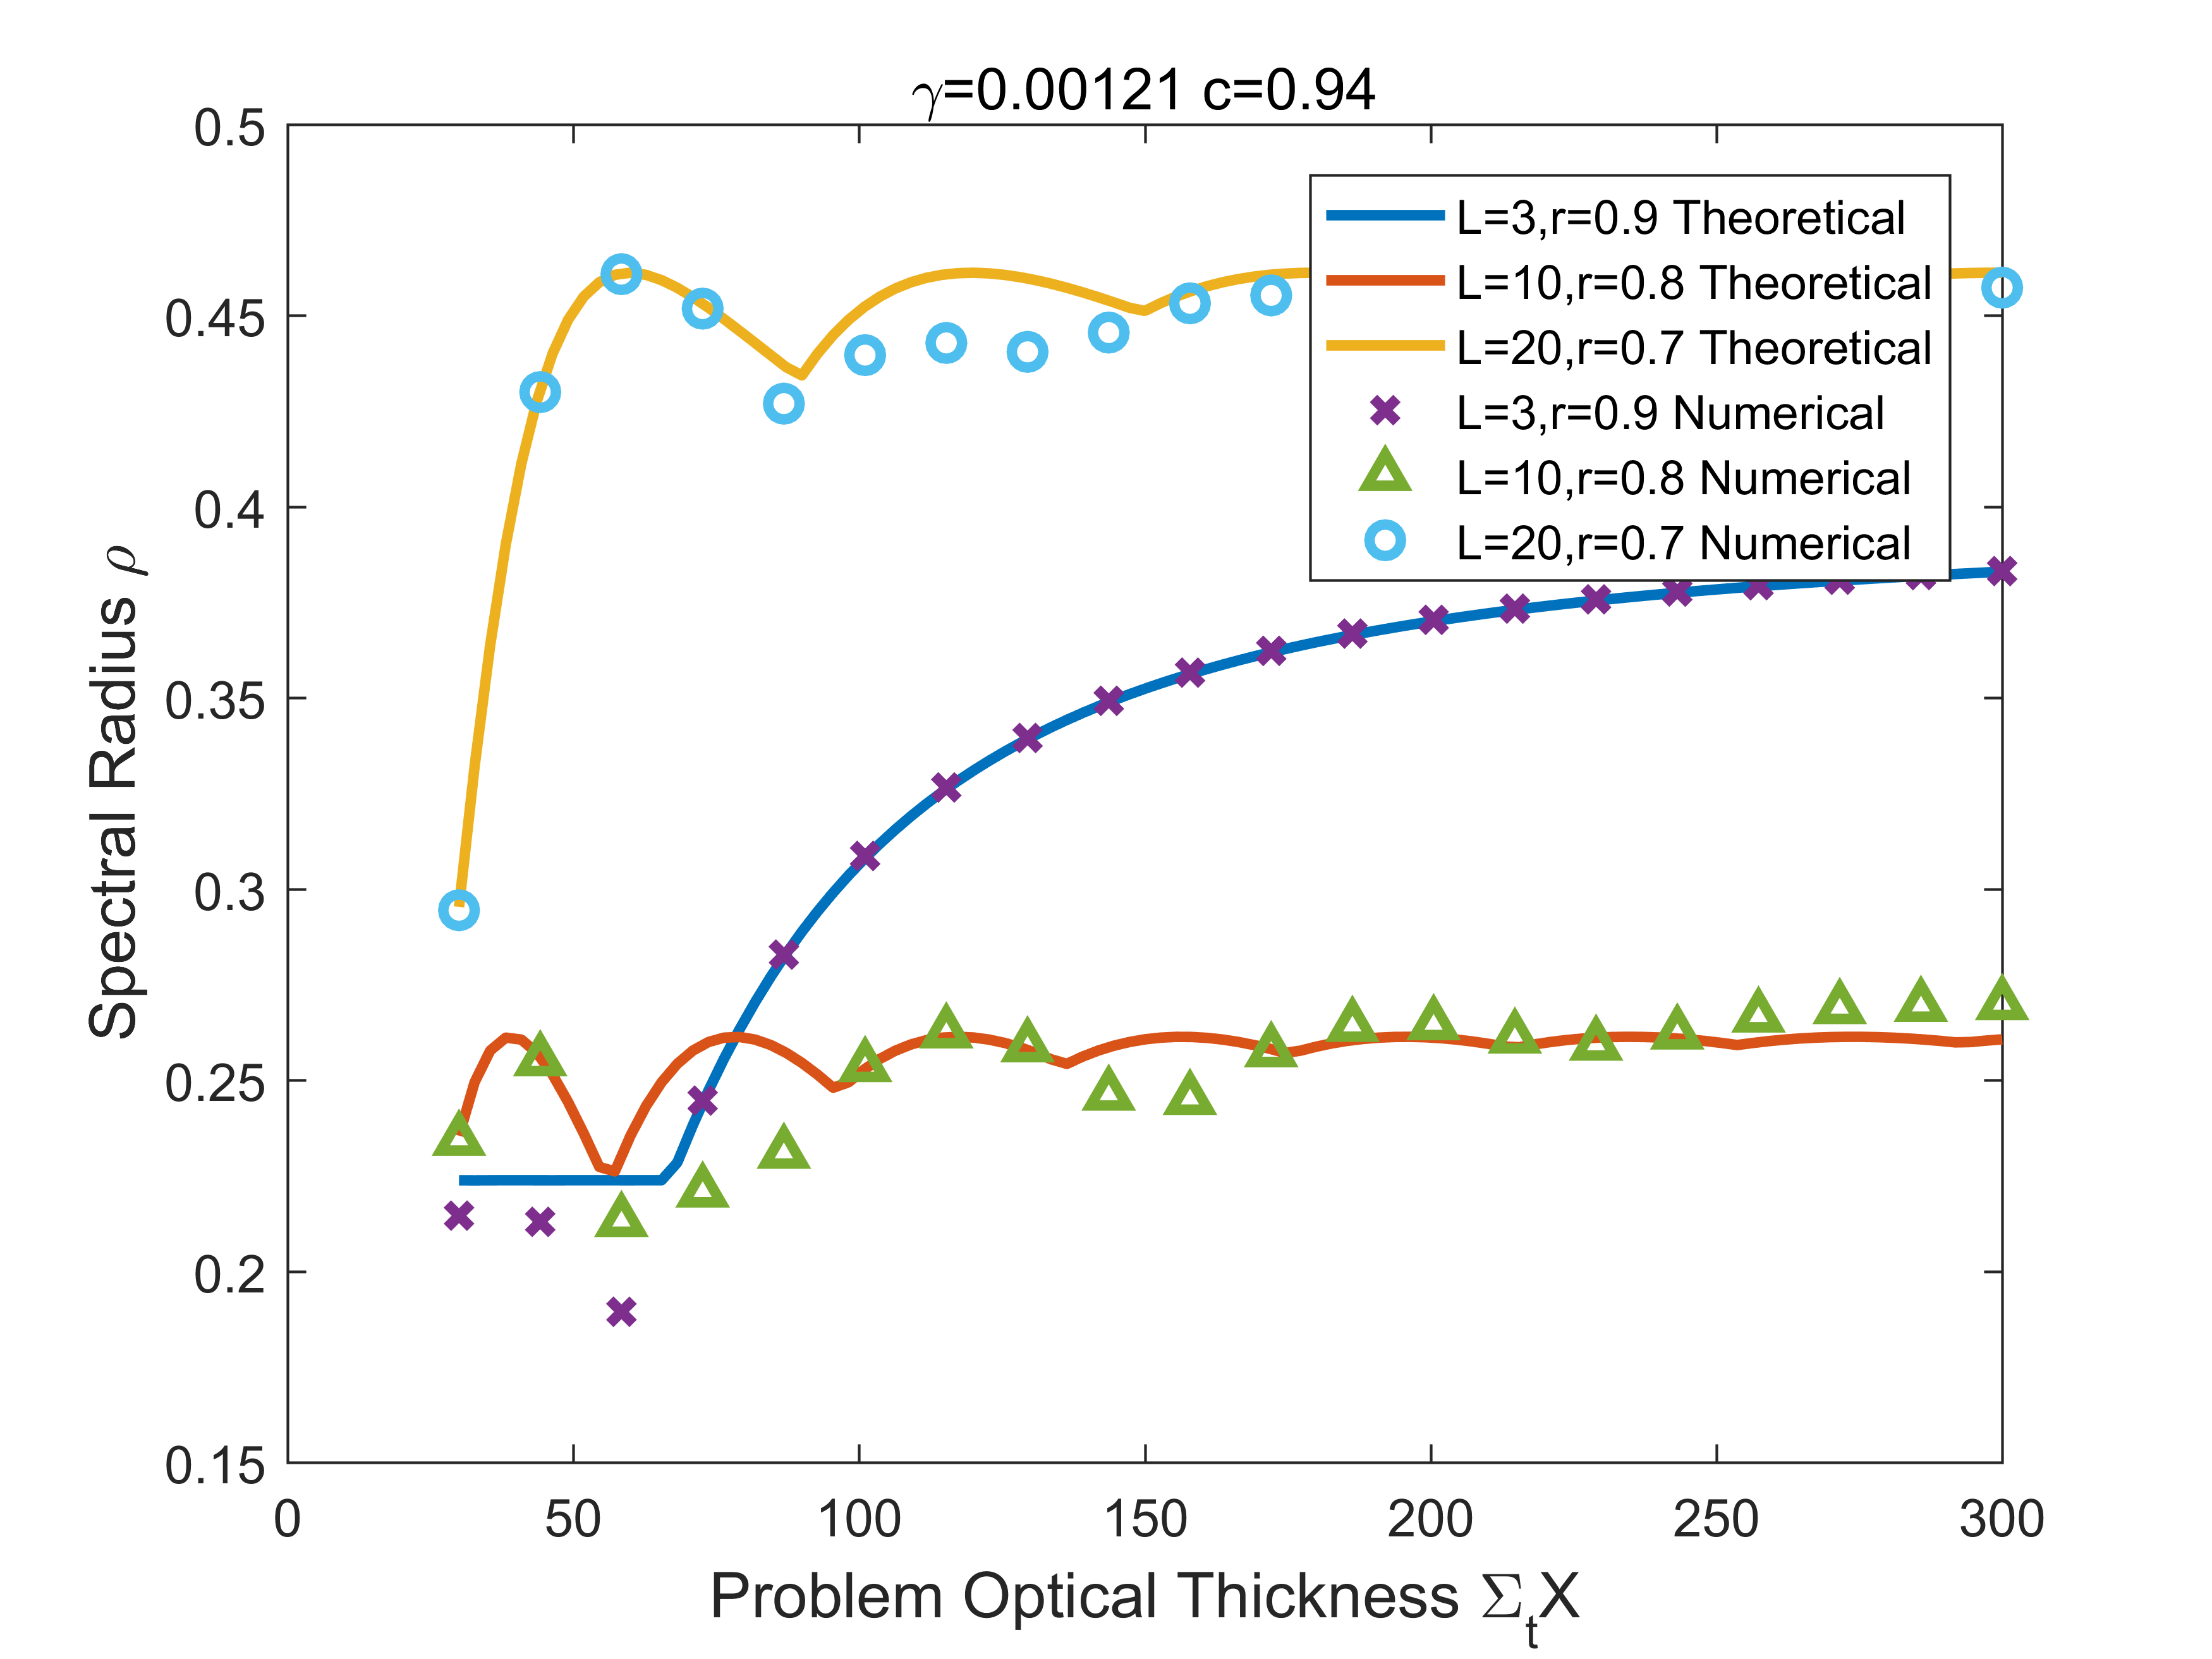
\includegraphics[width=\textwidth]{Texfile/Figure/TheovN_CT.png}
	\end{subfigure}
	\begin{subfigure}[t]{0.4\textwidth}
		\centering
		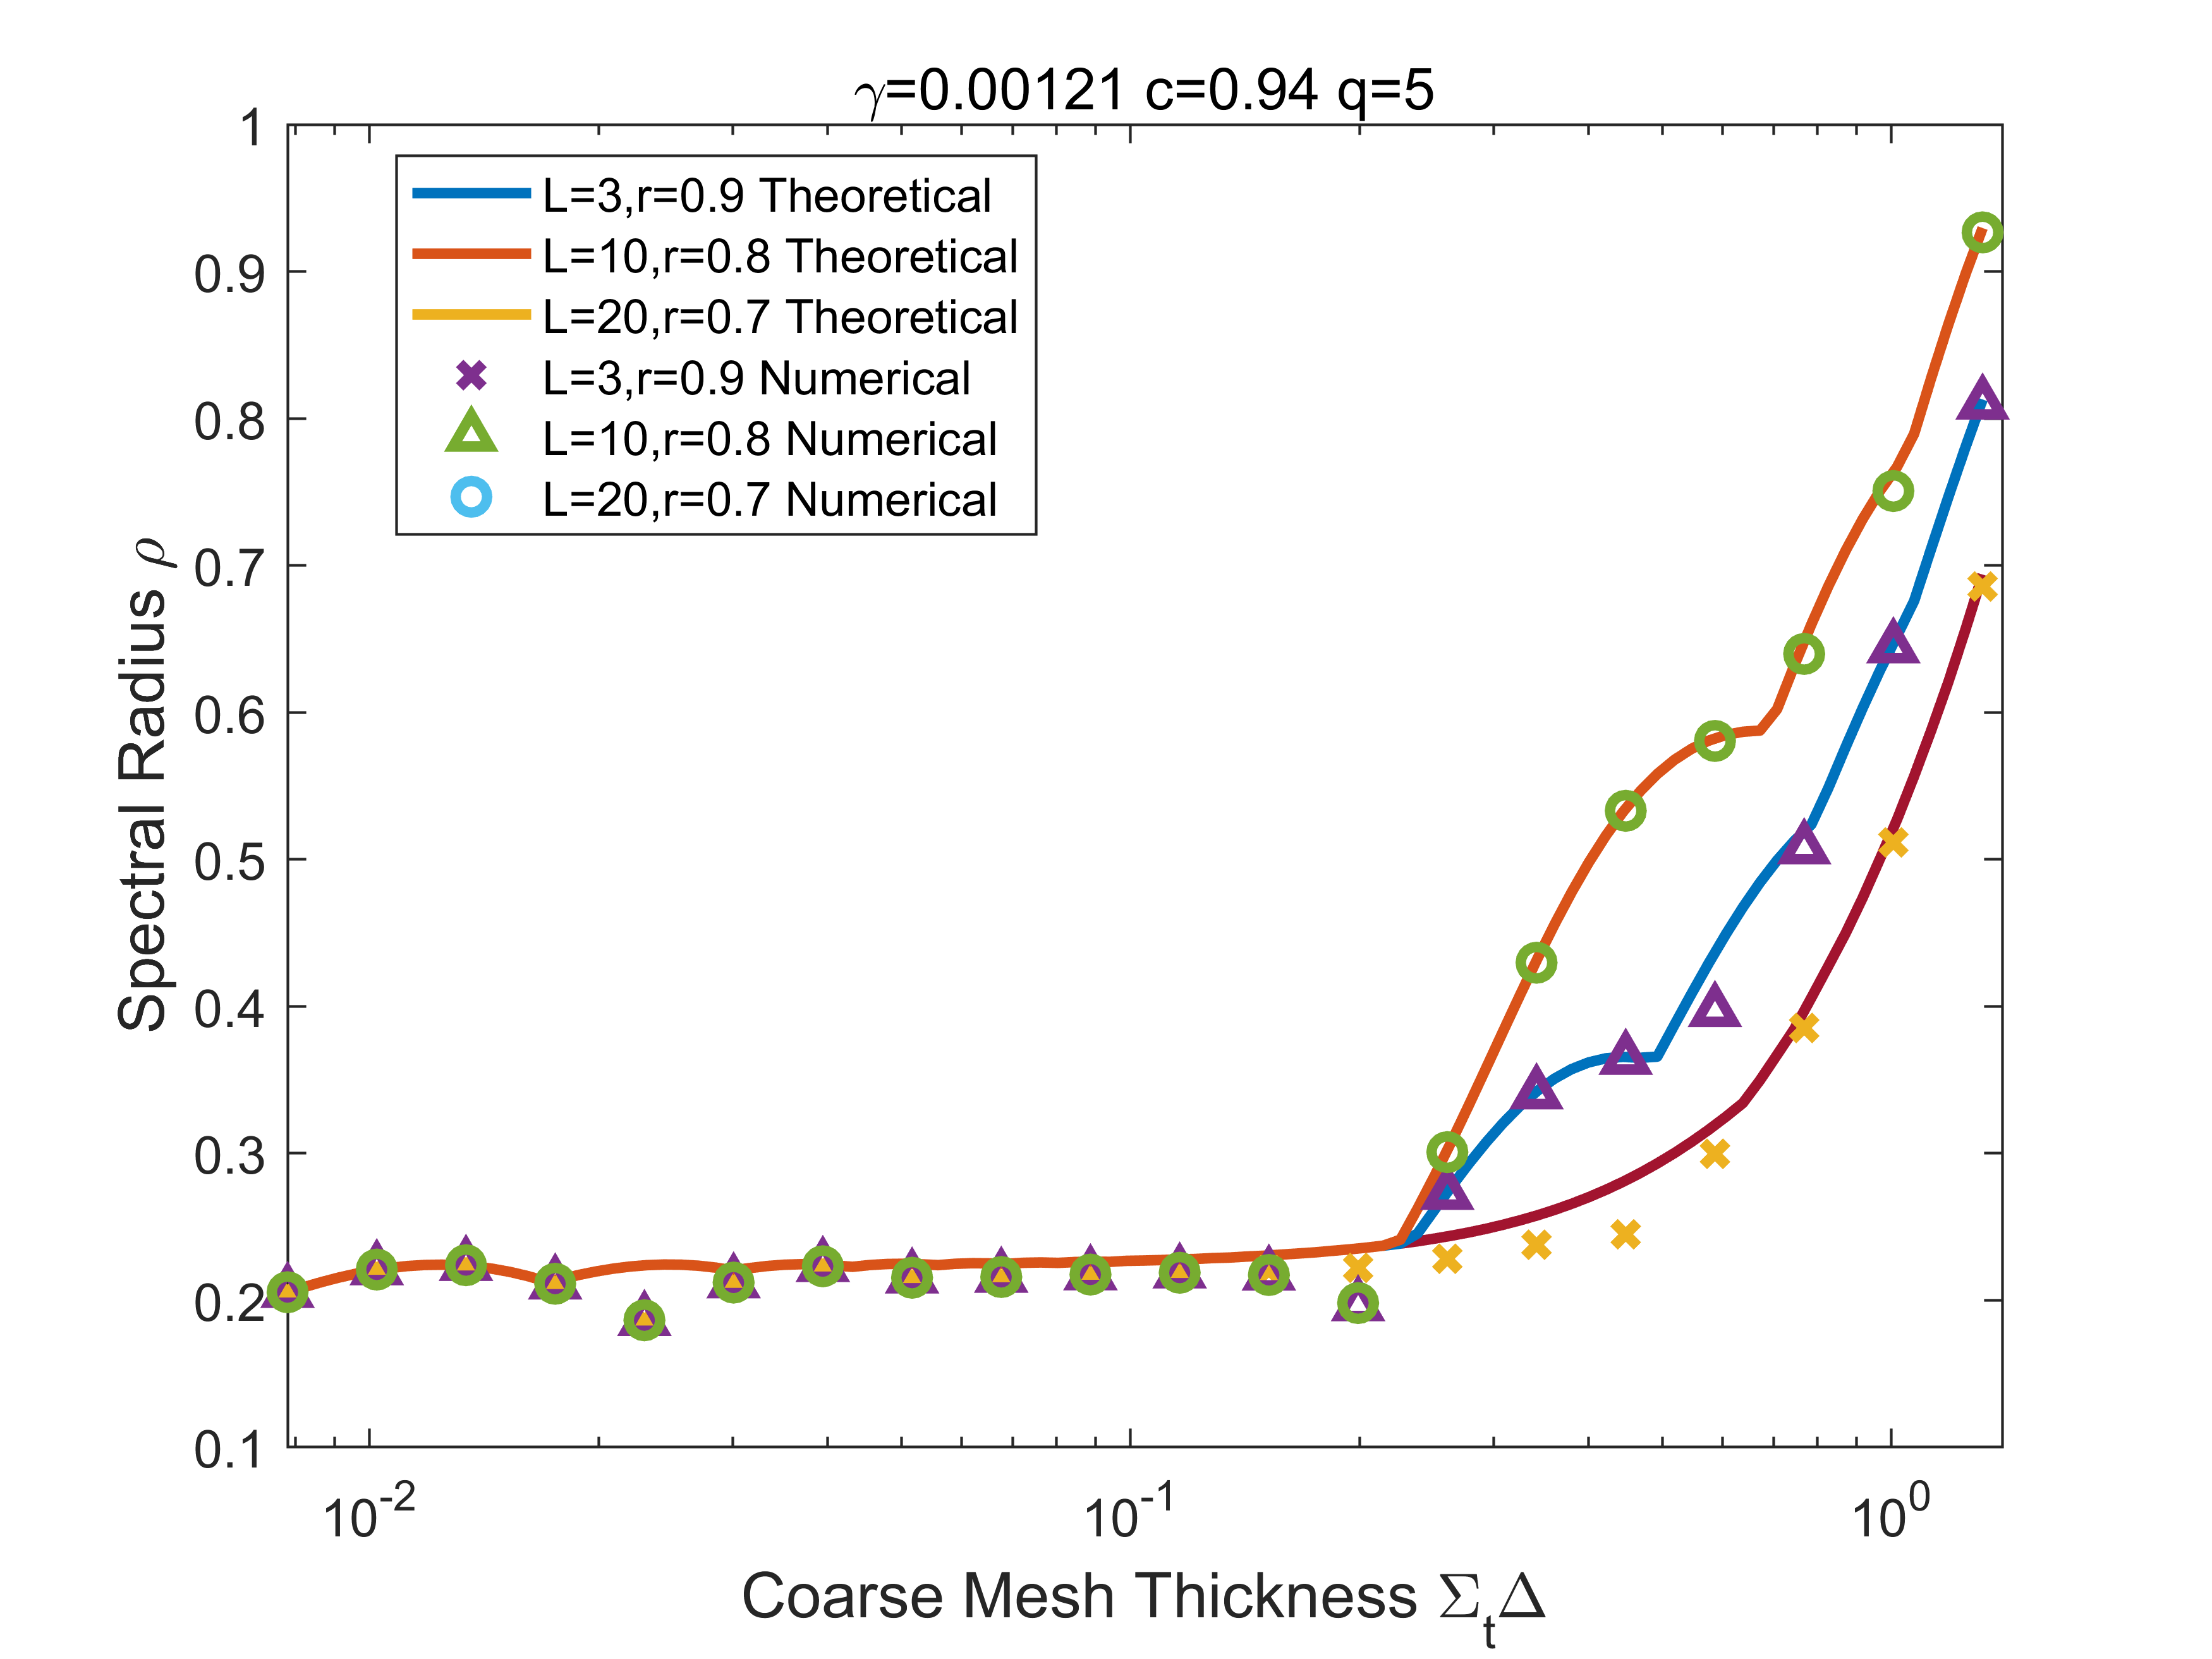
\includegraphics[width=\textwidth]{Texfile/Figure//TheovN_DT.png}
	\end{subfigure}
\end{figure} 

\vspace{-1.5em}
\begin{itemize}
    \item $L$,$r$ are randomly selected to make validation convincing. 
    \vspace{-0.5em}
    \item Wave shape of spectral radius indicates that the effect of partial convergence are problem dependent.
    \vspace{-0.5em}
    \item Fourier analysis predictions agree well with the numerical results from a test code.
\end{itemize}   
\end{frame}


%%%%%%%%%%%%%%%%%%%%%%%%%%%%%%%%%%%%%%%%%%%%%%%%%%%%
\begin{frame}{Effect of Power Iteration Number}
\vspace{-1em}
 \begin{figure}
	\centering
	\captionsetup[subfigure]{justification=centering}
	\begin{subfigure}[t]{0.4\textwidth}
		\centering
 		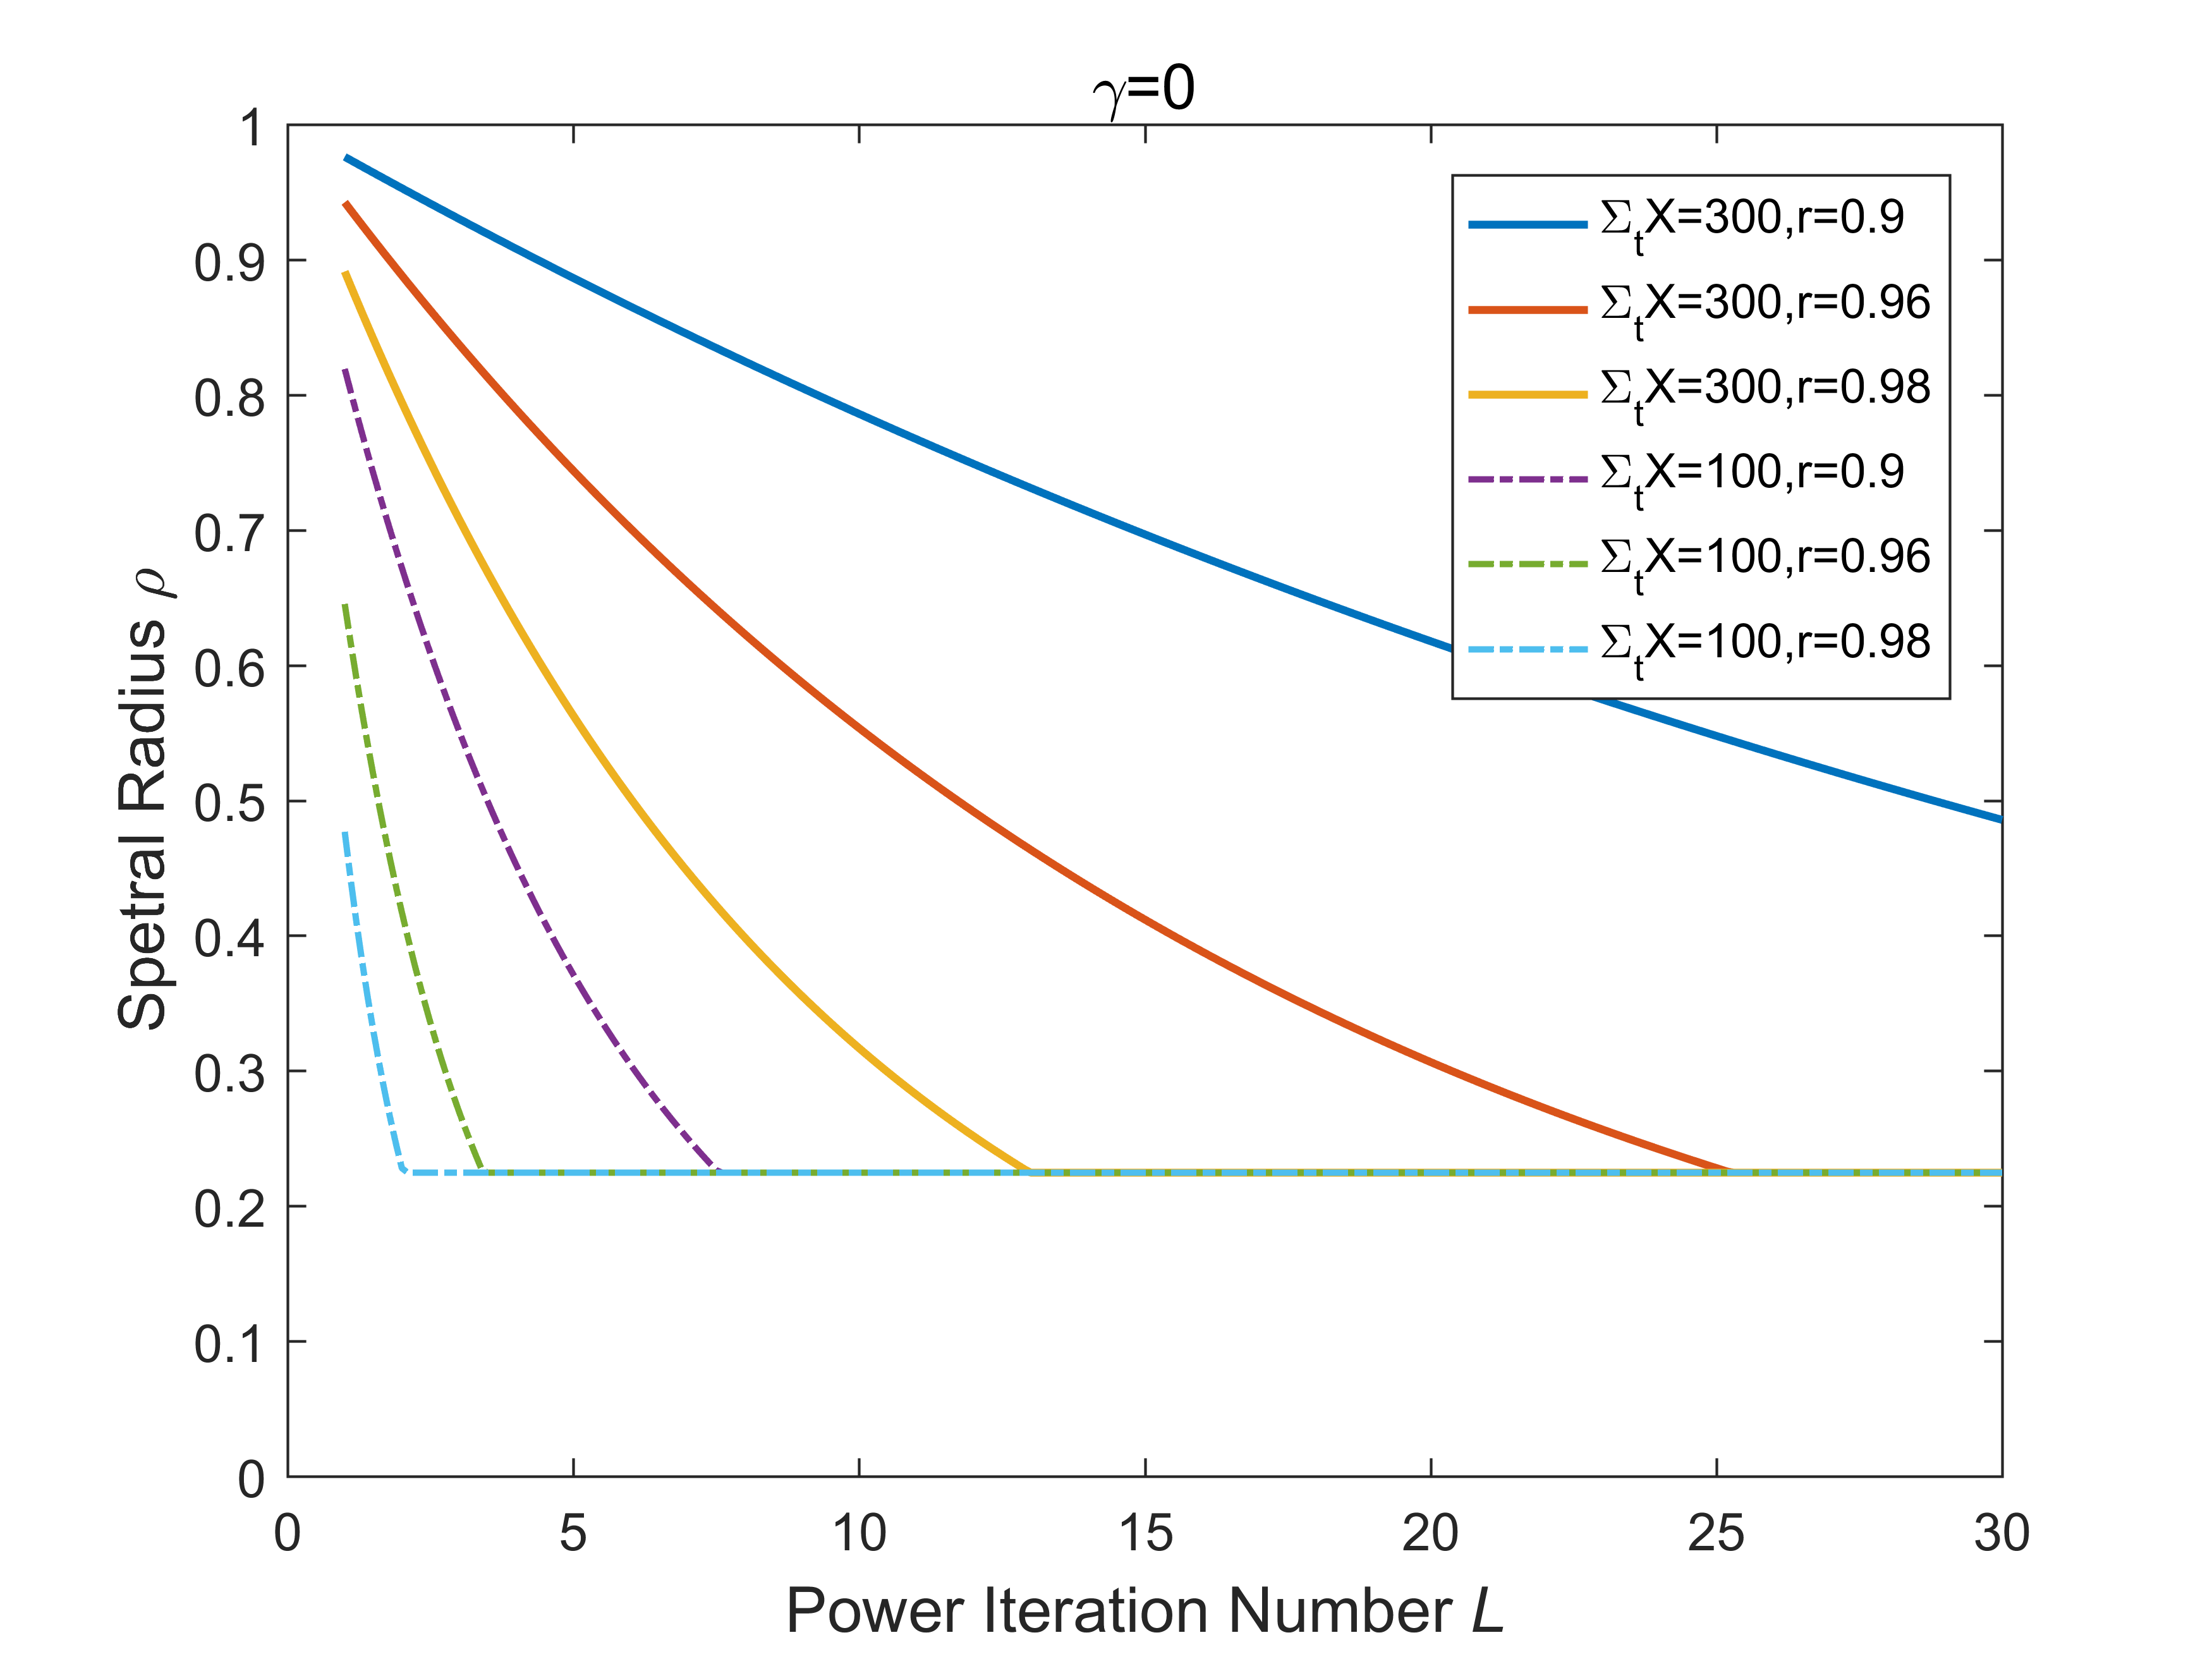
\includegraphics[width=\textwidth]{Texfile/Figure/noFeedback.png}
	\end{subfigure}
	\begin{subfigure}[t]{0.4\textwidth}
		\centering
		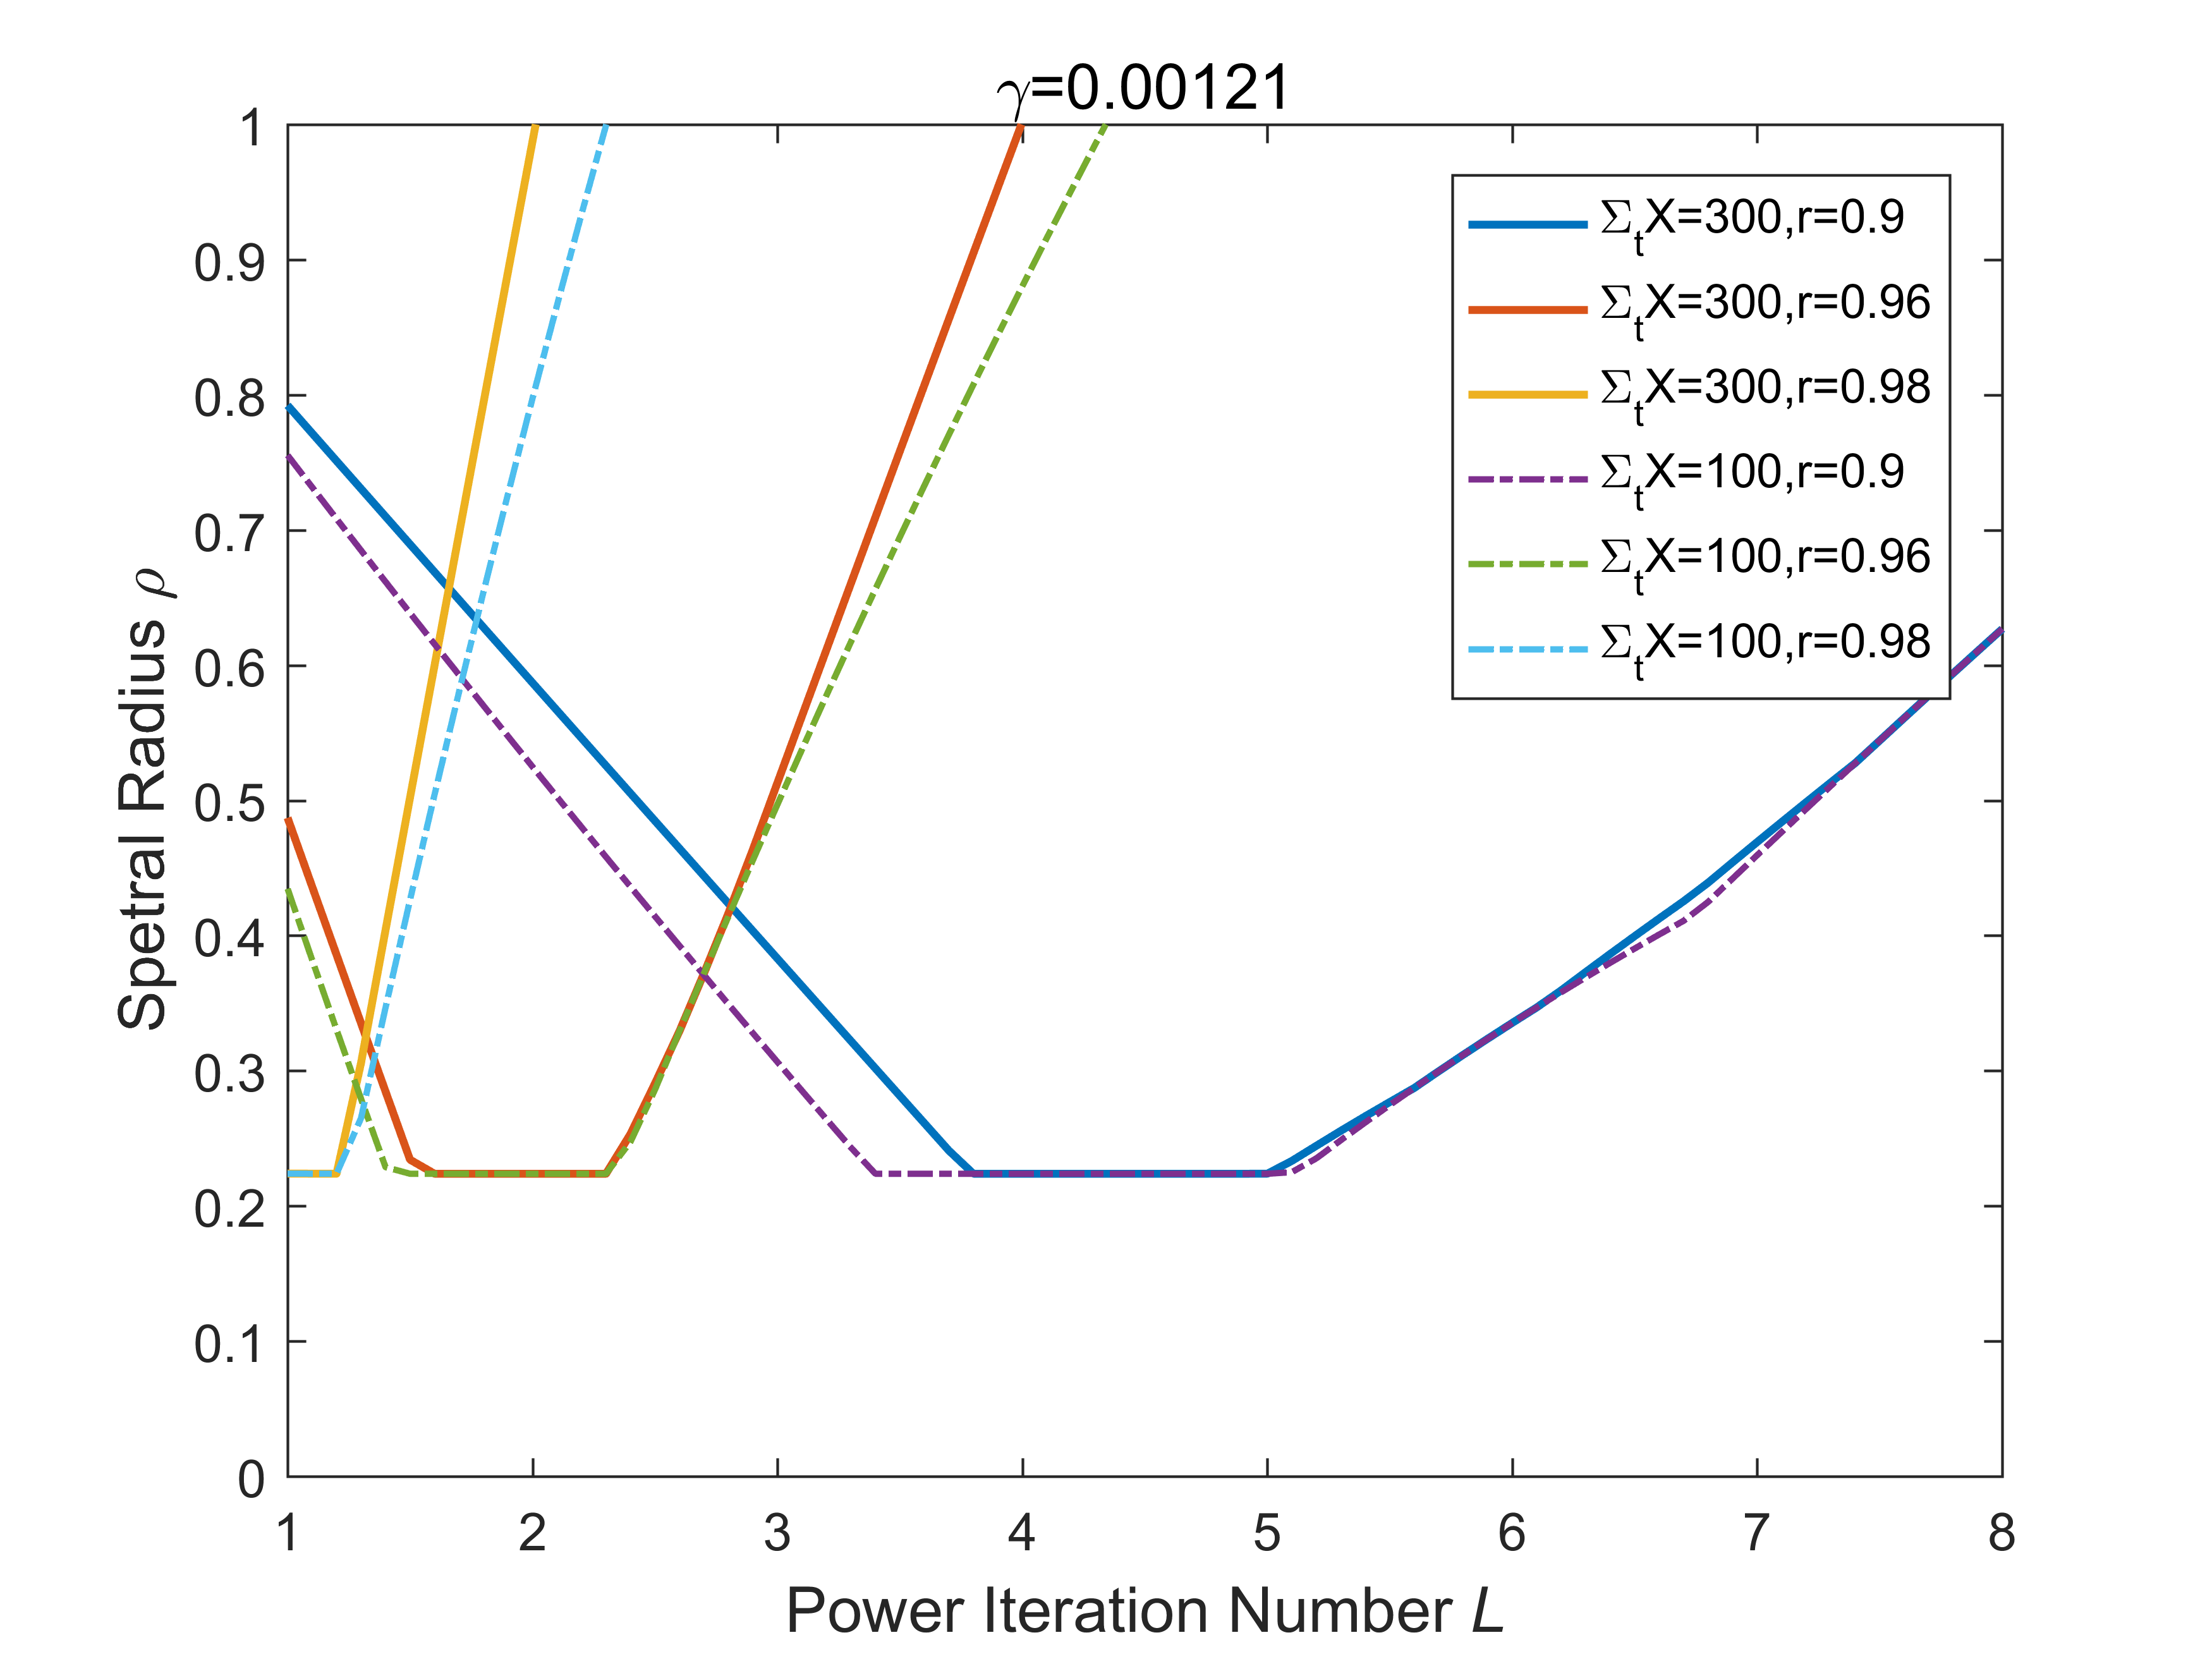
\includegraphics[width=\textwidth]{Texfile/Figure/Feedback_n.png}
	\end{subfigure}
\end{figure} 
\vspace{-1.5em}
\begin{itemize}
    \item Tightening the convergence of NDA by increasing the power iteration number or aggressiveness of Wielandt Shift will stablize the problem without feedback.
    \vspace{-0.7em}
    \item However, it will make the Picard scheme become more stable first, then more unstable till unconverged (similiar with the relaxation).
    \vspace{-0.7em}
    \item Near-optimal partial convergence exists but is problem-dependent.
\end{itemize}   
\end{frame}
% \begin{frame}{Effect of Power Iteration Number (Cont'd)}
% \vspace{-1em}
%  \begin{figure}
% 	\centering
% 	\captionsetup[subfigure]{justification=centering}
% 	\begin{subfigure}[t]{0.4\textwidth}
% 		\centering
%  		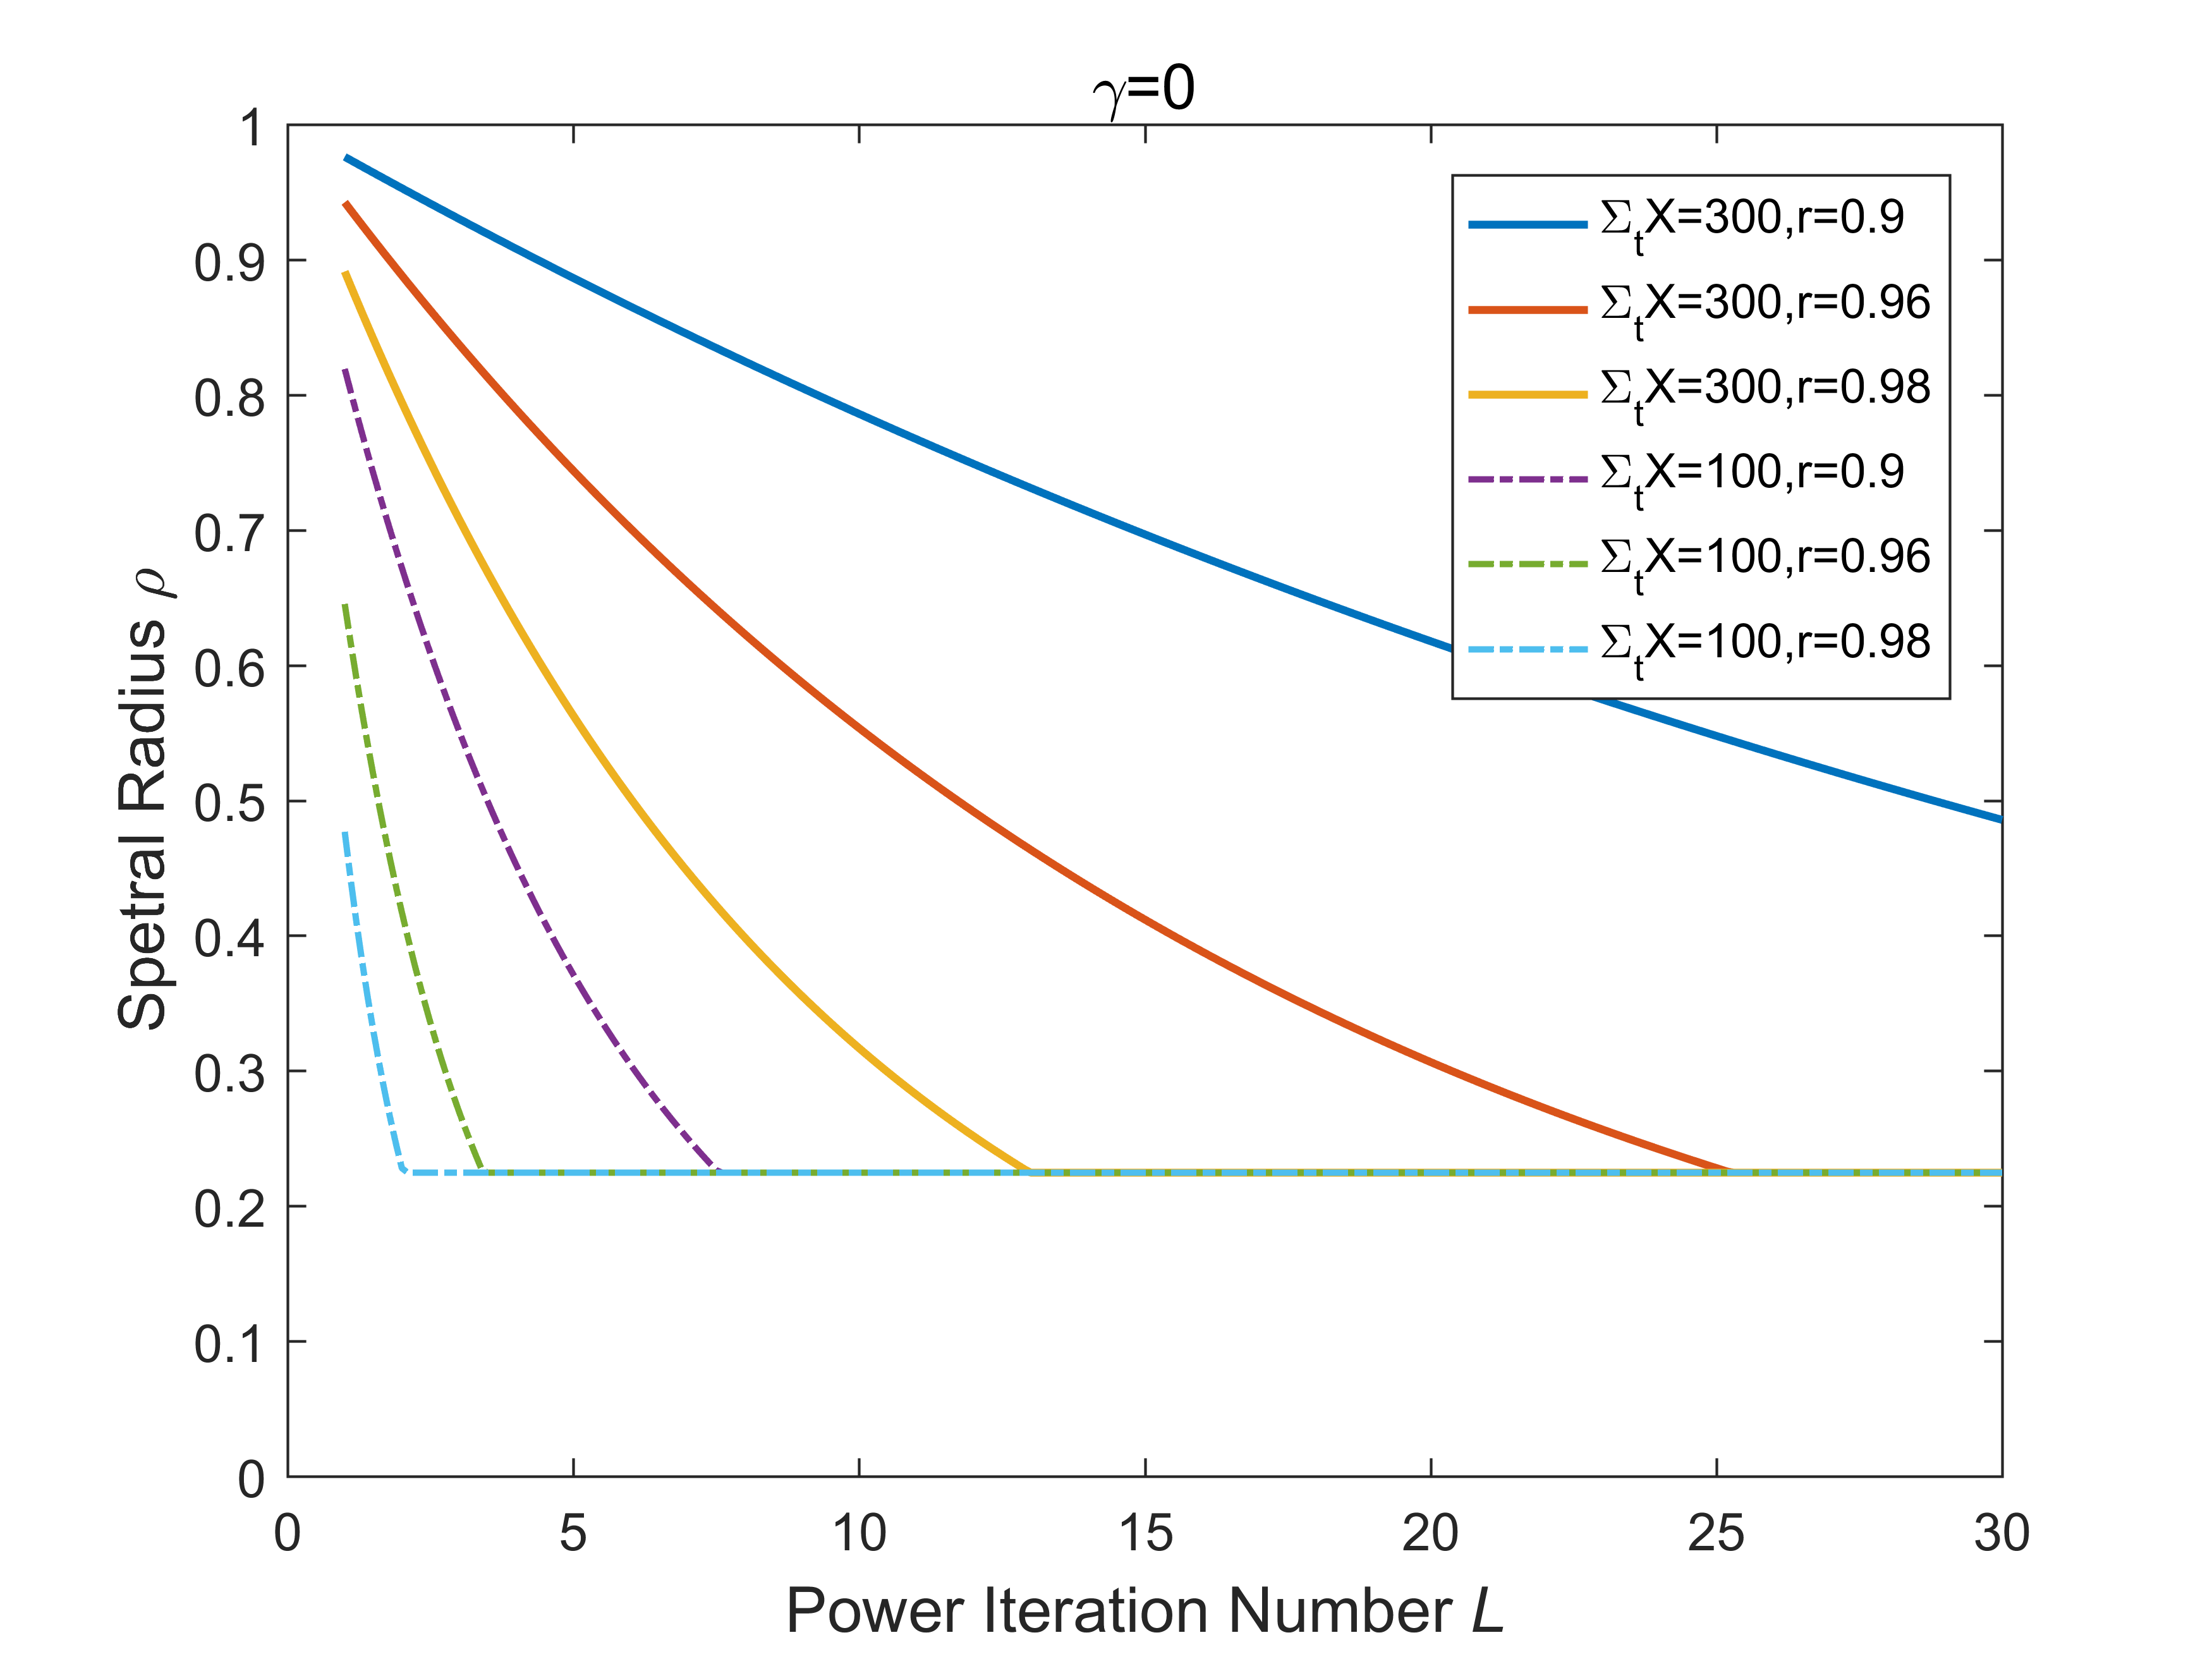
\includegraphics[width=\textwidth]{Texfile/Figure/noFeedback.png}
% 	\end{subfigure}
% 	\begin{subfigure}[t]{0.4\textwidth}
% 		\centering
% 		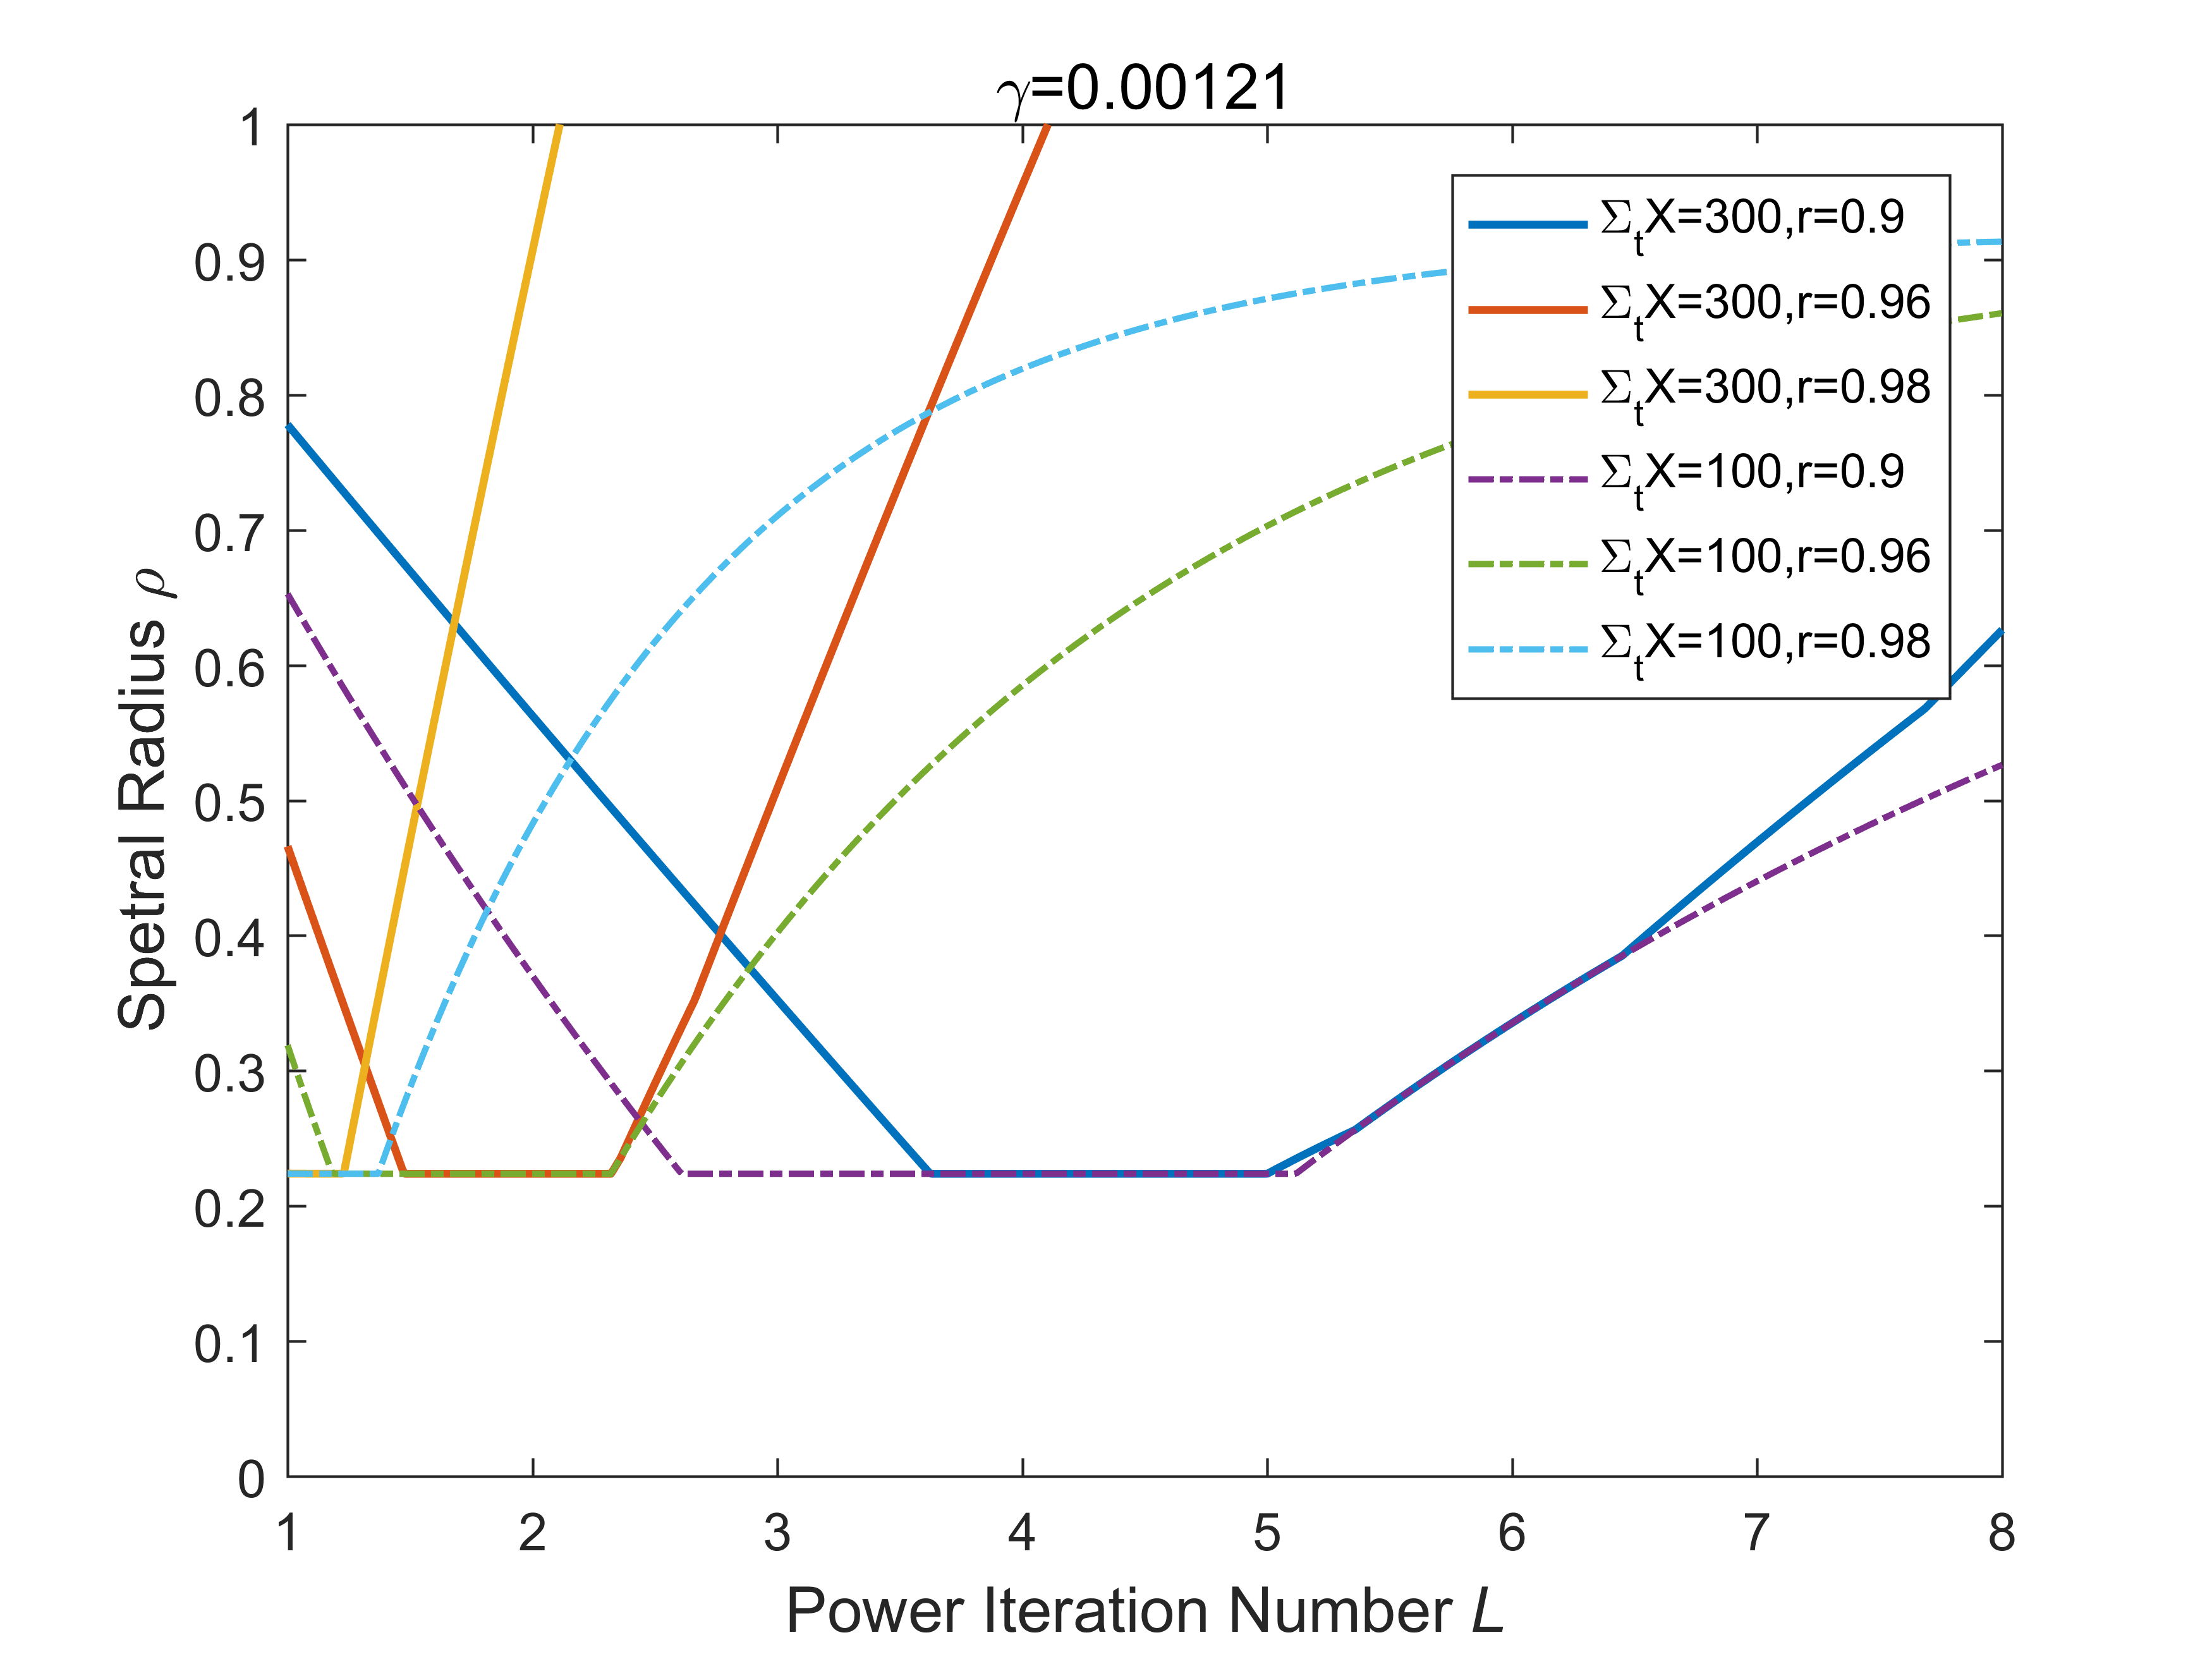
\includegraphics[width=\textwidth]{Texfile/Figure/Feedback.png}
% 	\end{subfigure}
% \end{figure} 
% \vspace{-1.5em}
% \begin{itemize}
%     \item \textbf{0.2247} can be achieved with partial convergence for problem with $\Sigma_tX=300$.
%     \vspace{-0.7em}
%     \item \textbf{Takeaway}: Try to fully converge in non-feedback problem. 
%     \item \textbf{Takeaway}: Try not to fully converge the NDA (CMFD) in feedback problem.
% \end{itemize}   
% \end{frame}
%%%%%%%%%%%%%%%%%%%%%%%%%%%%%%%%%%%%%%%%%%%%%%%%%%%%%%%%%%%%%%%%%%%%%%%%%%%%%%%%%%%%%%%%%%%%%%%%%%%%%%%%%%%%%%%%%%%%%%%%%%%%%%%%
\subsection{Relationship between Partial Convergence and Relaxation}
%%%%%%%%%%%%%%%%%%%%%%%%%%%%%%%%%%%%%%%%%%%%%%%%%%%%
\begin{frame}{Fourier Analysis Result of Fully Converged Nonlinear Diffusion Acceleration with Flux Relaxation}

\begin{itemize}
    \item Flux relaxation is applied when using coarse mesh flux to update the transport solution by:
    \begin{equation}
        \phi(x)=\beta\phi_j+(1-\beta)\phi(x)
    \end{equation}
    \item Final Expression:
    \begin{align}\label{eqns:four-theta}
     \theta(\omega)=
        \begin{cases}
        \bSr{1-\beta-\gamma}f_{TS}(\omega)
        +\beta\bBr{f_{NDA}(\omega)-\frac{3\gamma}{\omega^2}f_{TS}(\omega)} \;, &\text{continuous problem}\\
            \max \blr{eig\bSr{\mathbf{T}(\omega)}}\;, \text{discretized problem}
        \end{cases}
\end{align}

    where:
    \begin{align}
    \mathbf{T}(\omega)=\tilde{\mathbf{H}}(\omega)(1-\gamma)-\beta\mathbf{1}\frac{3\Sigma_t\Delta(e^{i\Sigma_t\Delta\omega}-1)\tilde{\mathbf{G}}+\gamma3(\Sigma_t\Delta)^2\frac{\mathbf{1}^T}{q}\tilde{\mathbf{H}}}{2-2cos(\Sigma_t\Delta\omega)} \label{eq:eror_tr_mtx}
    \end{align} 
\end{itemize}  
\end{frame}

%%%%%%%%%%%%%%%%%%%%%%%%%%%%%%%%%%%%%%%%%%%%%%%%%%%%%%%%%%%%%%%%%%%%%%%%%%%%%%%%%%%%%%%%%%%%%%%%%%%%%%%%%%%%%%%%%%%%%%%%%%%%%%%%
\begin{frame}{Relation between Partial Convergence and Flux Relaxation}
\vspace{-1em}
 \begin{figure}
	\centering
	\captionsetup[subfigure]{justification=centering}
	\begin{subfigure}[t]{0.45\textwidth}
		\centering
 		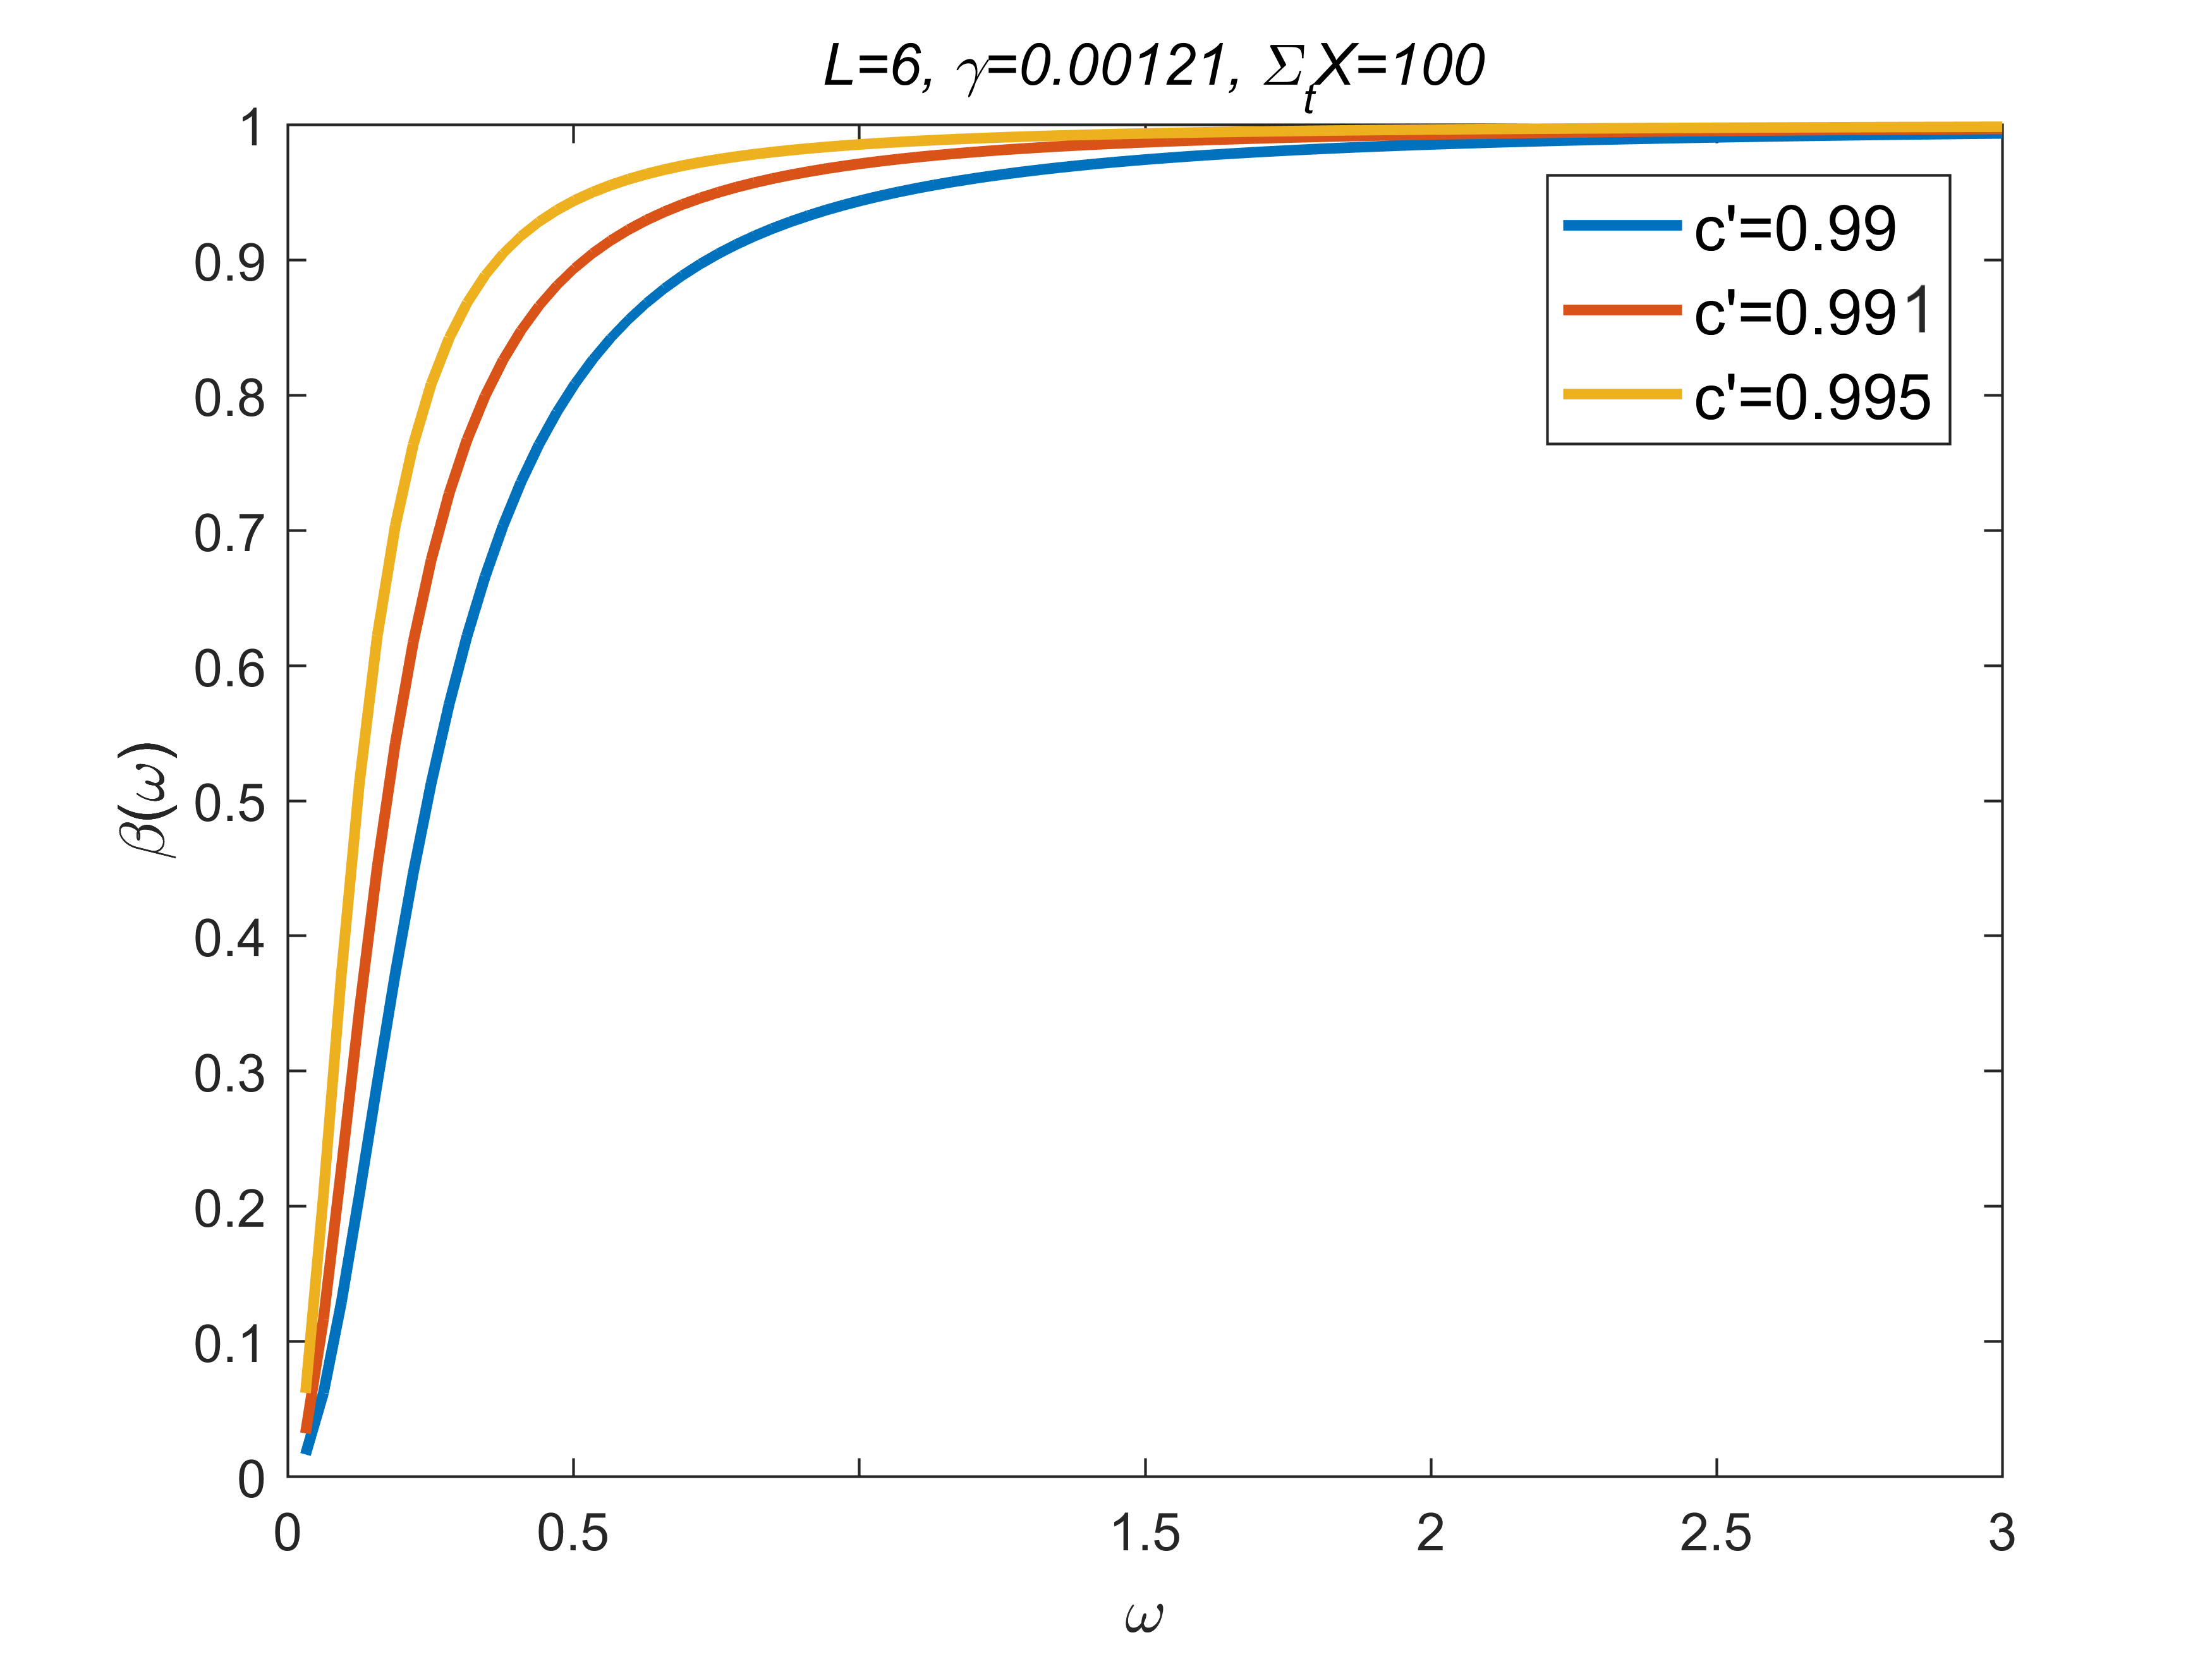
\includegraphics[width=\textwidth]{Texfile/Figure/betavomega.png}
	\end{subfigure}
	\begin{subfigure}[t]{0.45\textwidth}
		\centering
		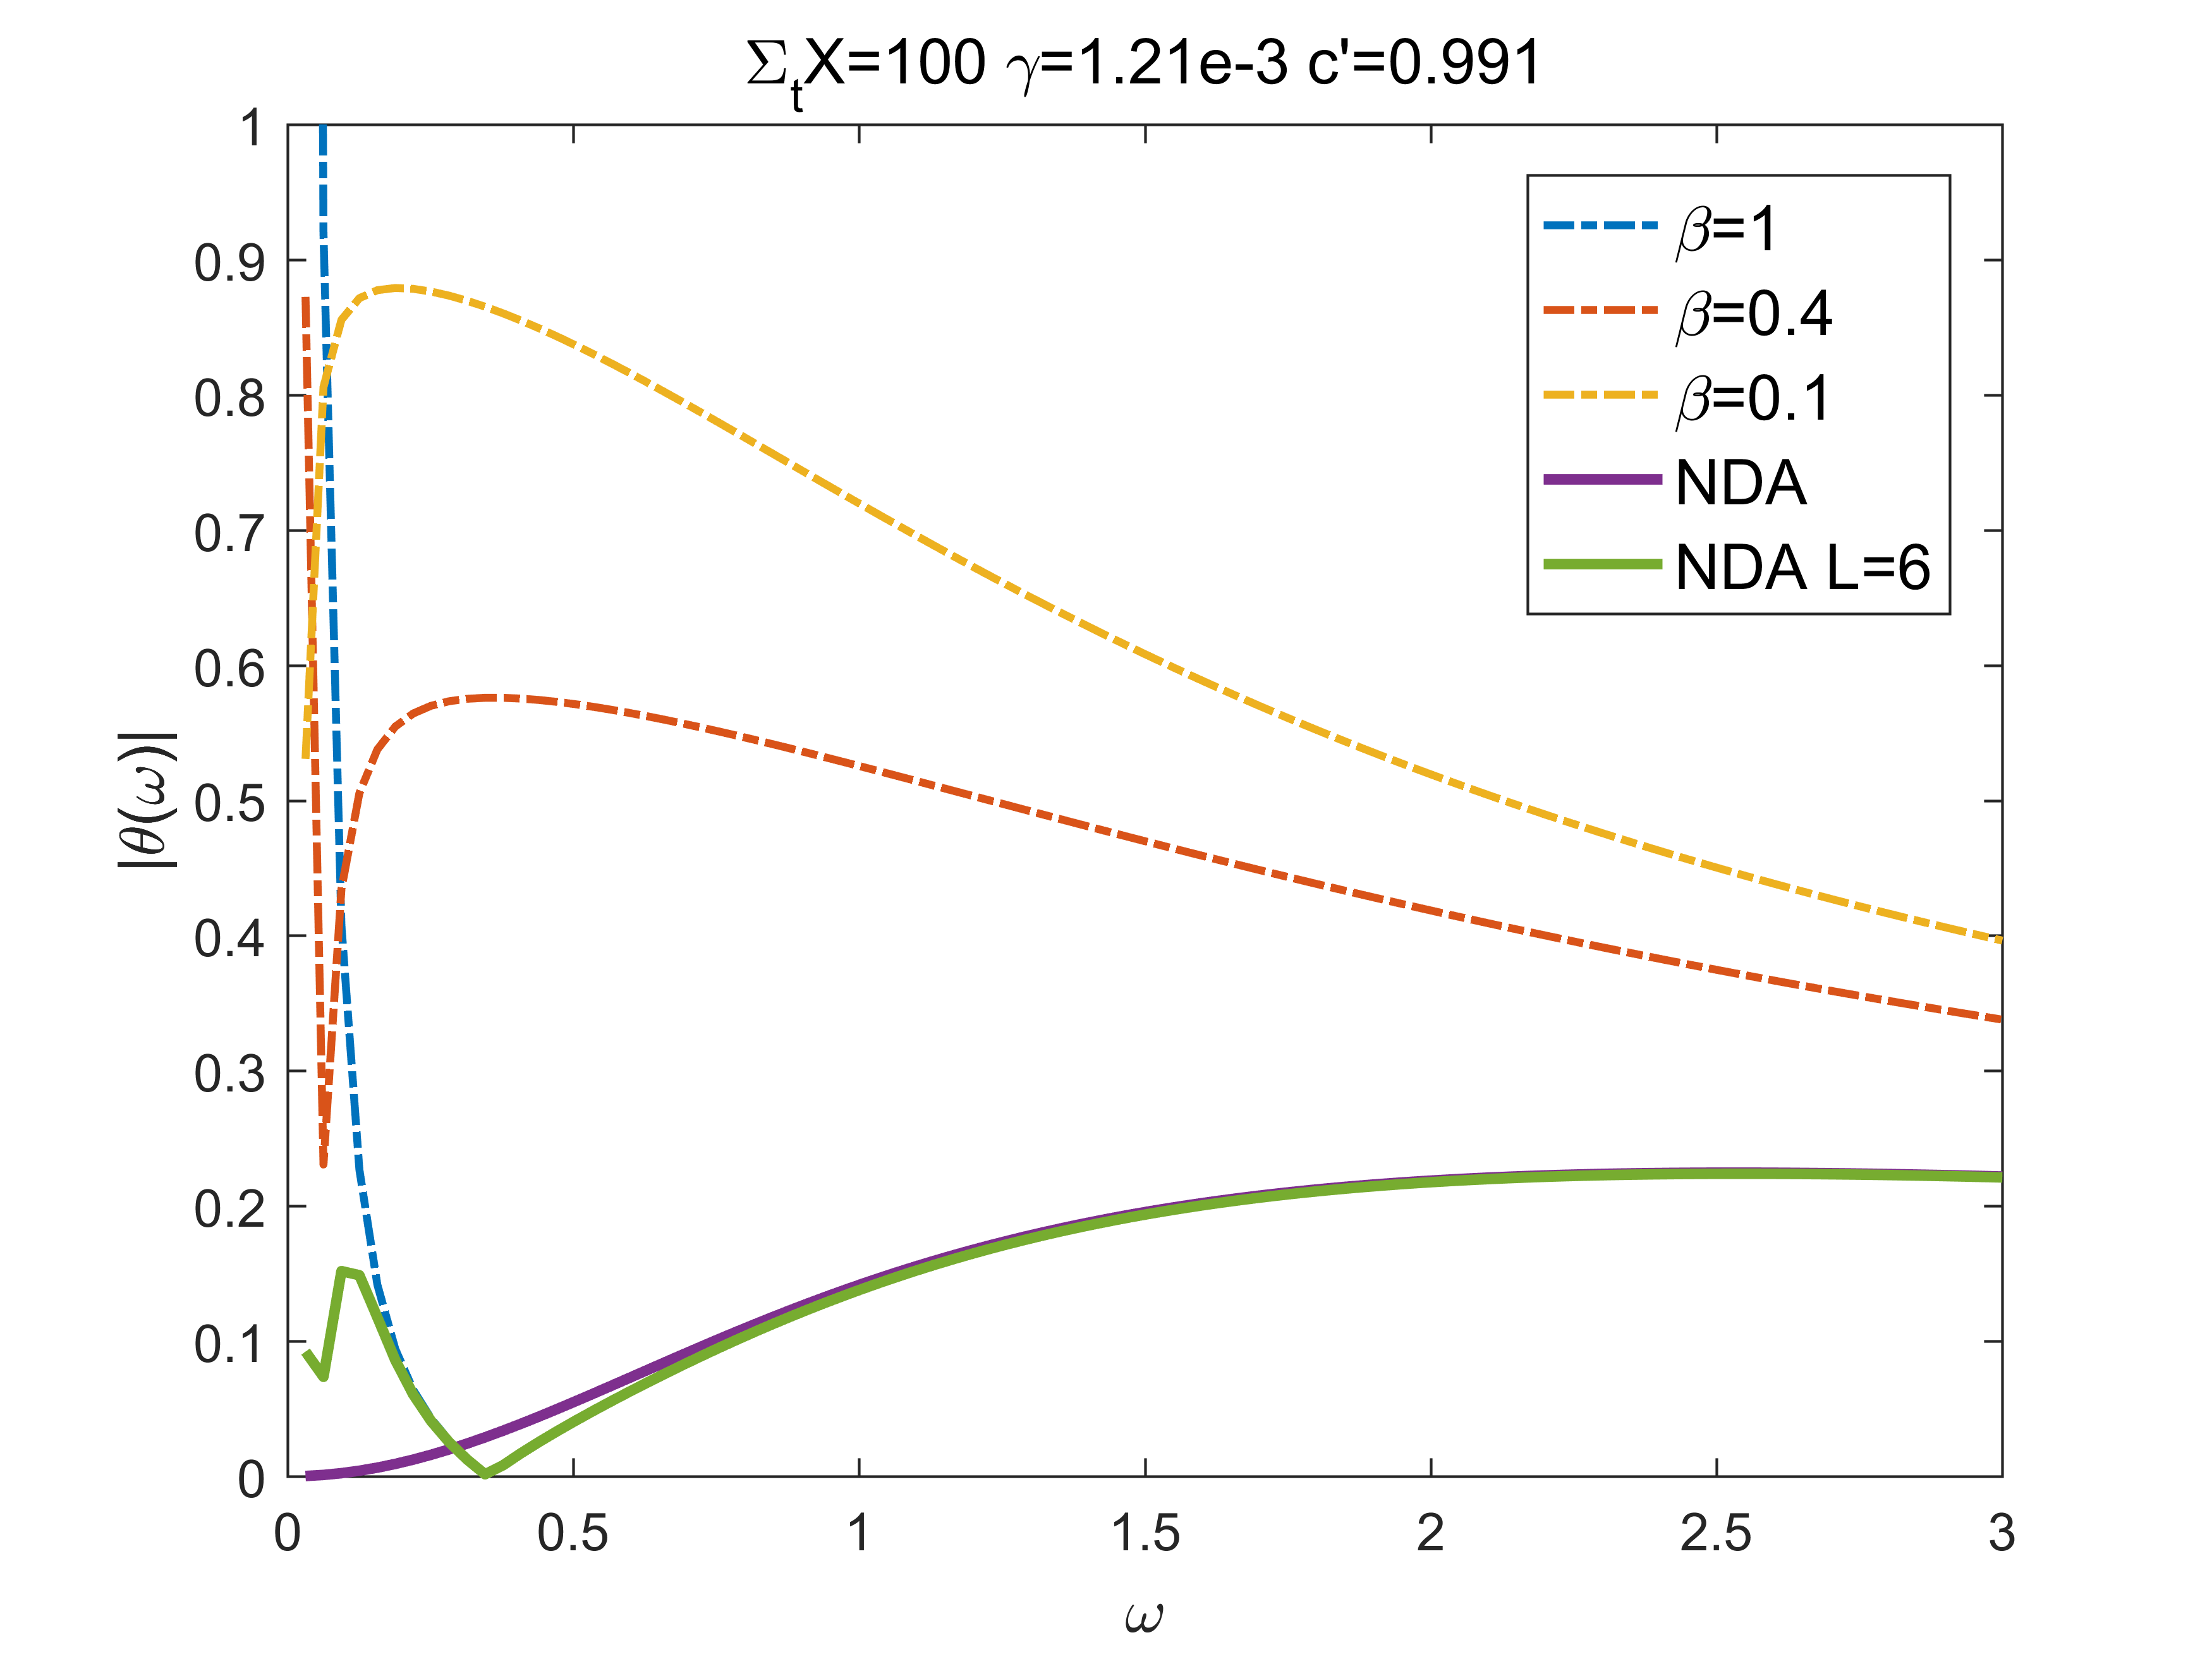
\includegraphics[width=\textwidth]{Texfile/Figure/rhovo_n.png}
	\end{subfigure}
\end{figure} 
\vspace{-1.5em}
\begin{itemize}
    \item Partial convergence induces the Fourier-frequency-dependent flux relaxation factor:
    \vspace{-0.5em}
    \begin{equation}\label{eq:betad}
        \beta(\omega)=1-\Lambda^L(\omega).
    \end{equation}\\
    \vspace{-1.2em}
    \item The relaxation is mainly imposed on the relatively flat Fourier error modes.
\end{itemize}
\end{frame}
%%%%%%%%%%%%%%%%%%%%%%%%%%%%%%%%%%%%%%%%%%%%%%%%%%%%%%%%%%%%%%%%%%%%%%%%%%%%%%%%%%%%%%%%%%%%%%%%%%%%%%%%%%%%%%%%%%%%%%%%%%%%%
\subsection{Near-Optimal Partial Convergence}
\begin{frame}{Derivation of the Near-Optimal Partial Convergence}
\vspace{-1em}
 \begin{itemize}
    \item Rewrite the expression for spectral radius as for continuous case:
    \begin{equation}
       \theta(\omega)=\bSr{1-\beta(\omega)-\gamma-\beta(\omega)\frac{3\gamma}{\omega^2}}f_{TS}(\omega)
        +\beta(\omega)f_{NDA} 
    \end{equation}
    \item For relatively flat fourier modes, $f_{TS}(\omega)\approx 1$
    \item The near optimal partial convergence should make:
    \vspace{-0.2cm}
    \begin{equation}
        1-\beta(\omega)-\gamma-\beta(\omega)\frac{3\gamma}{\omega^2}\approx0
    \end{equation}
    \vspace{-1em}
    the near-optimal partial convergence in term of wielandt shift is:
    \begin{equation}\label{eq:opr}
        r=1-\frac{\left(1-\beta(\omega)\right)^{\frac{1}{L}}}{1-\left(1-\beta(\omega)\right)^{\frac{1}{L}}}\frac{\omega^2}{3(1-c)}.
    \end{equation}   
     \vspace{-1em}
\end{itemize}  
\end{frame}
%%%%%%%%%%%%%%%%%%%%%%%%%%%%%%%%%%%%%%%%%%%%%%%%%%%%%%%%%%%%%%%%%%%%%%%%%%%%%%%%%%%%%%%%%%%%%%%%%
\begin{frame}{Test of Near-Optimal Partial Convergence}
\vspace{-1em}
 \begin{figure}
	\centering
	\captionsetup[subfigure]{justification=centering}
	\begin{subfigure}[t]{0.45\textwidth}
		\centering
 		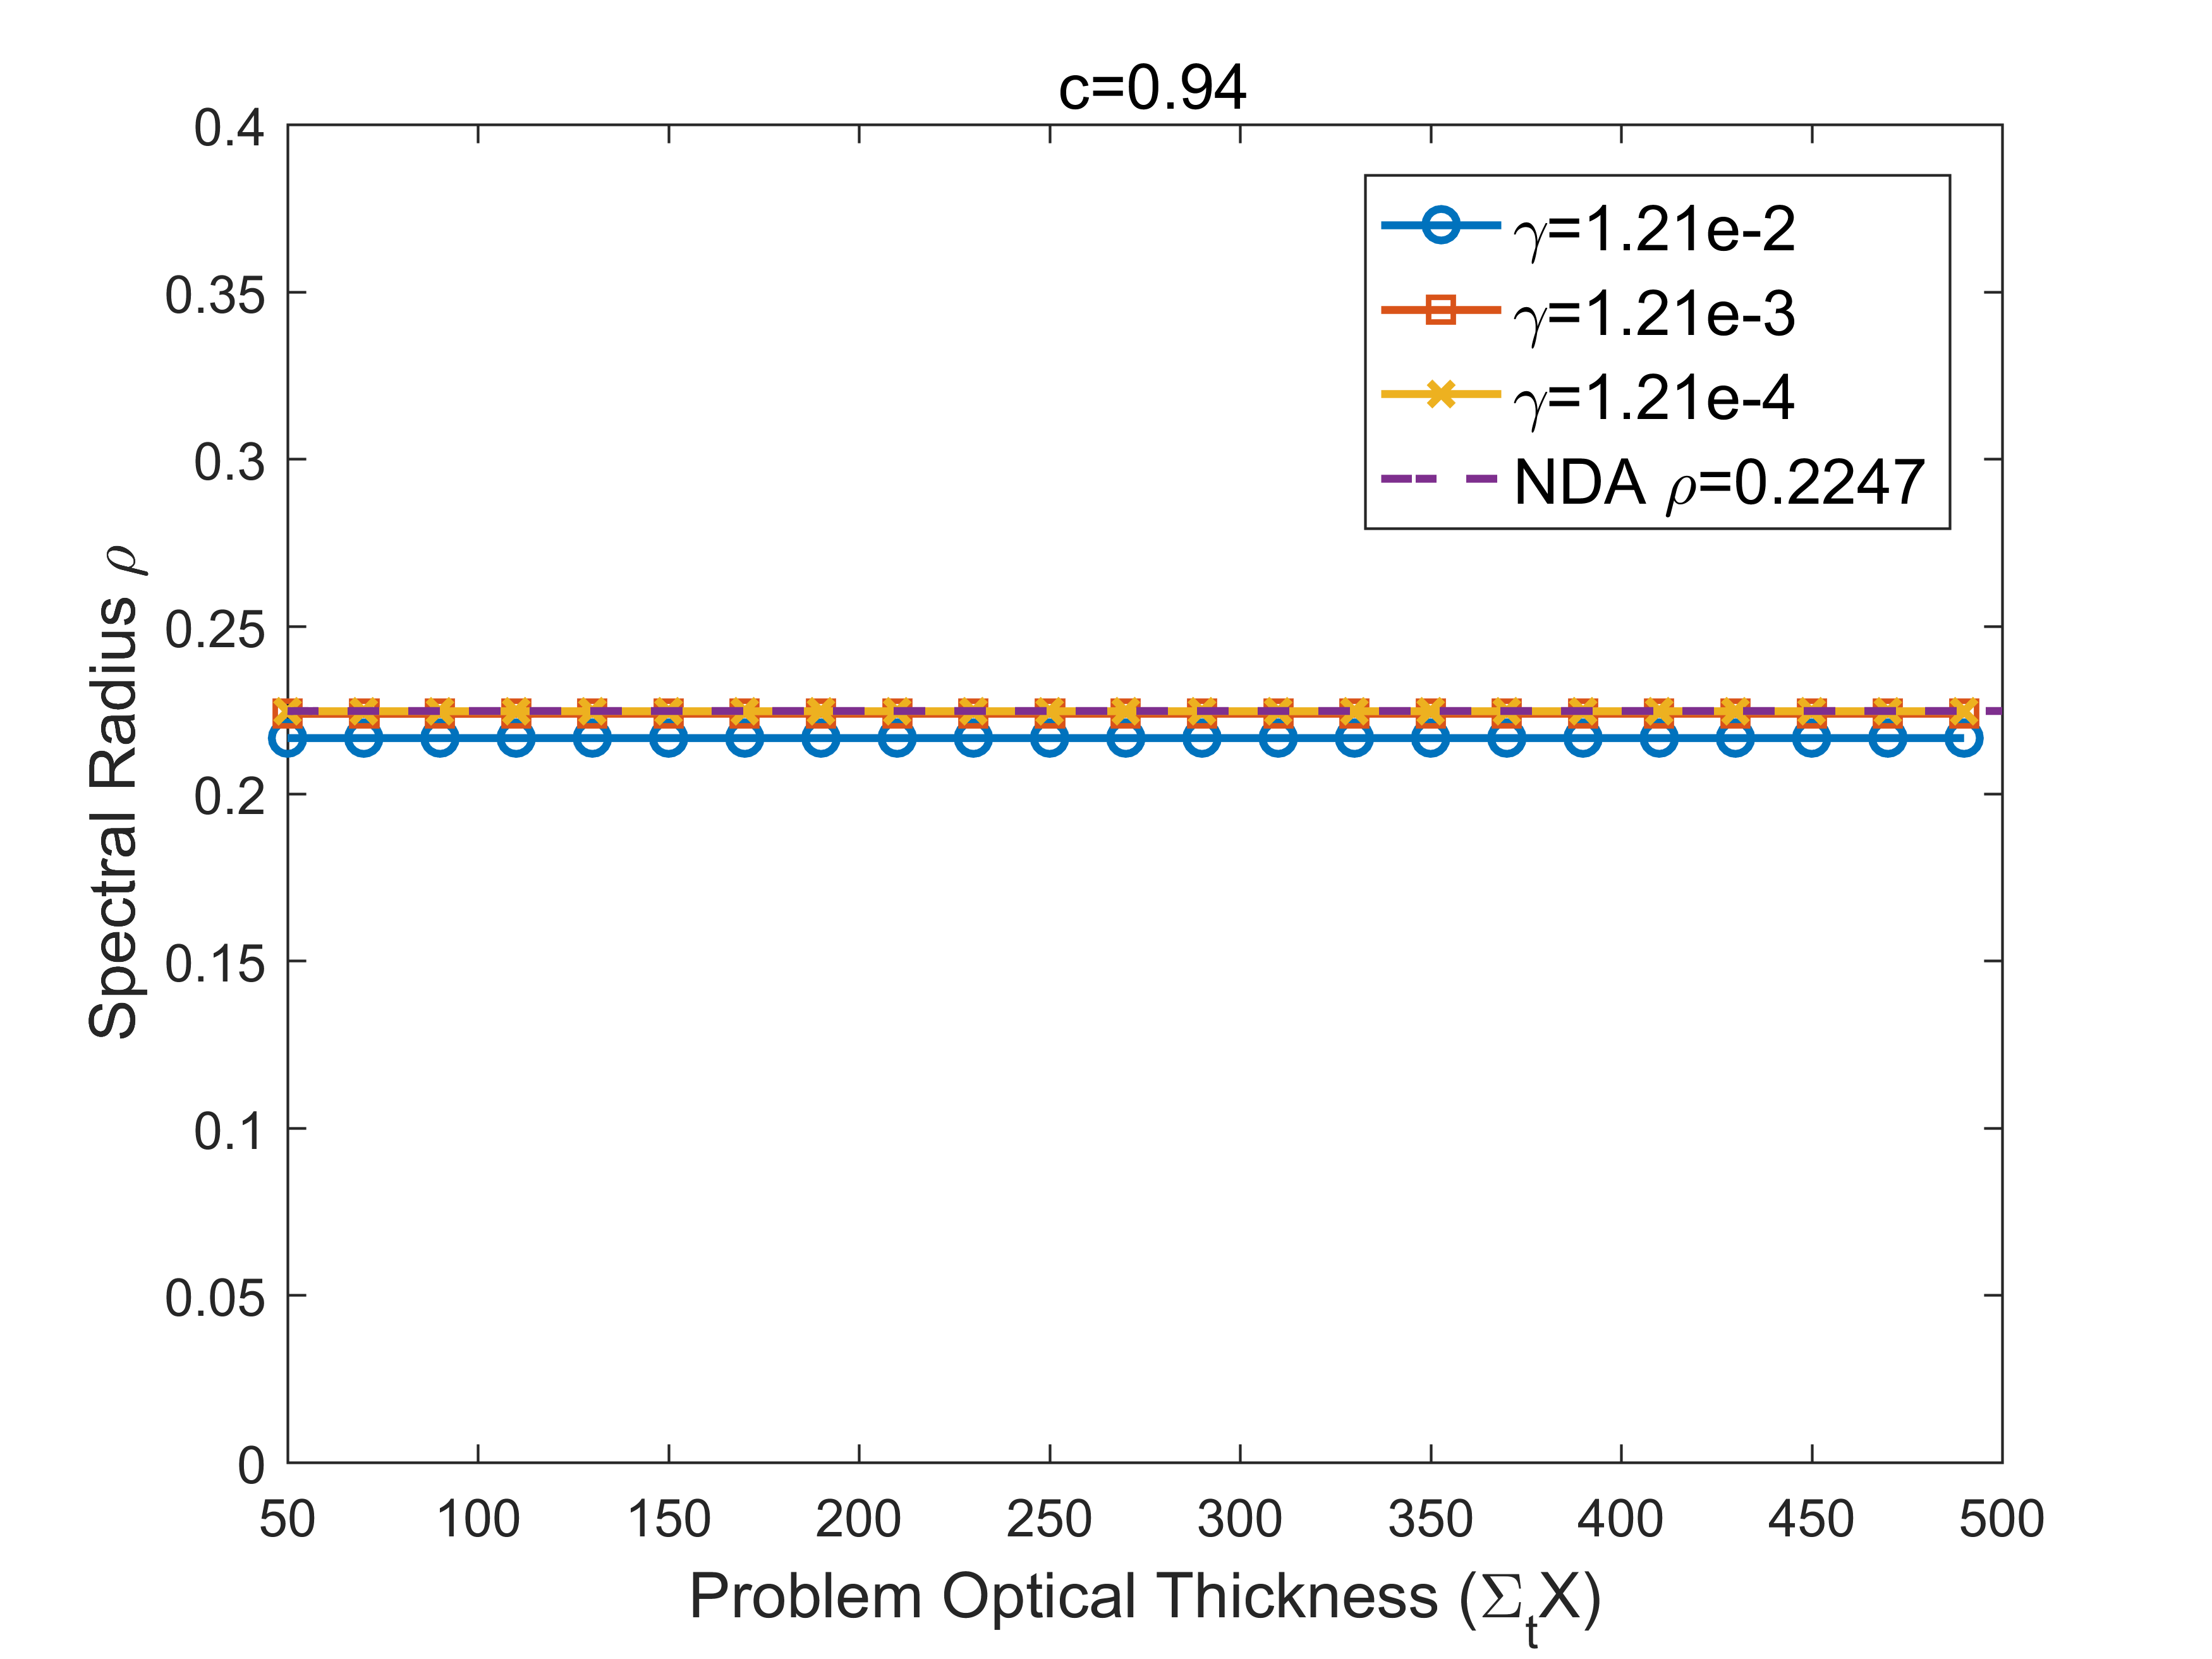
\includegraphics[width=\textwidth]{Texfile/Figure/NDAoptimal.png}
	\end{subfigure}
	\begin{subfigure}[t]{0.45\textwidth}
		\centering
		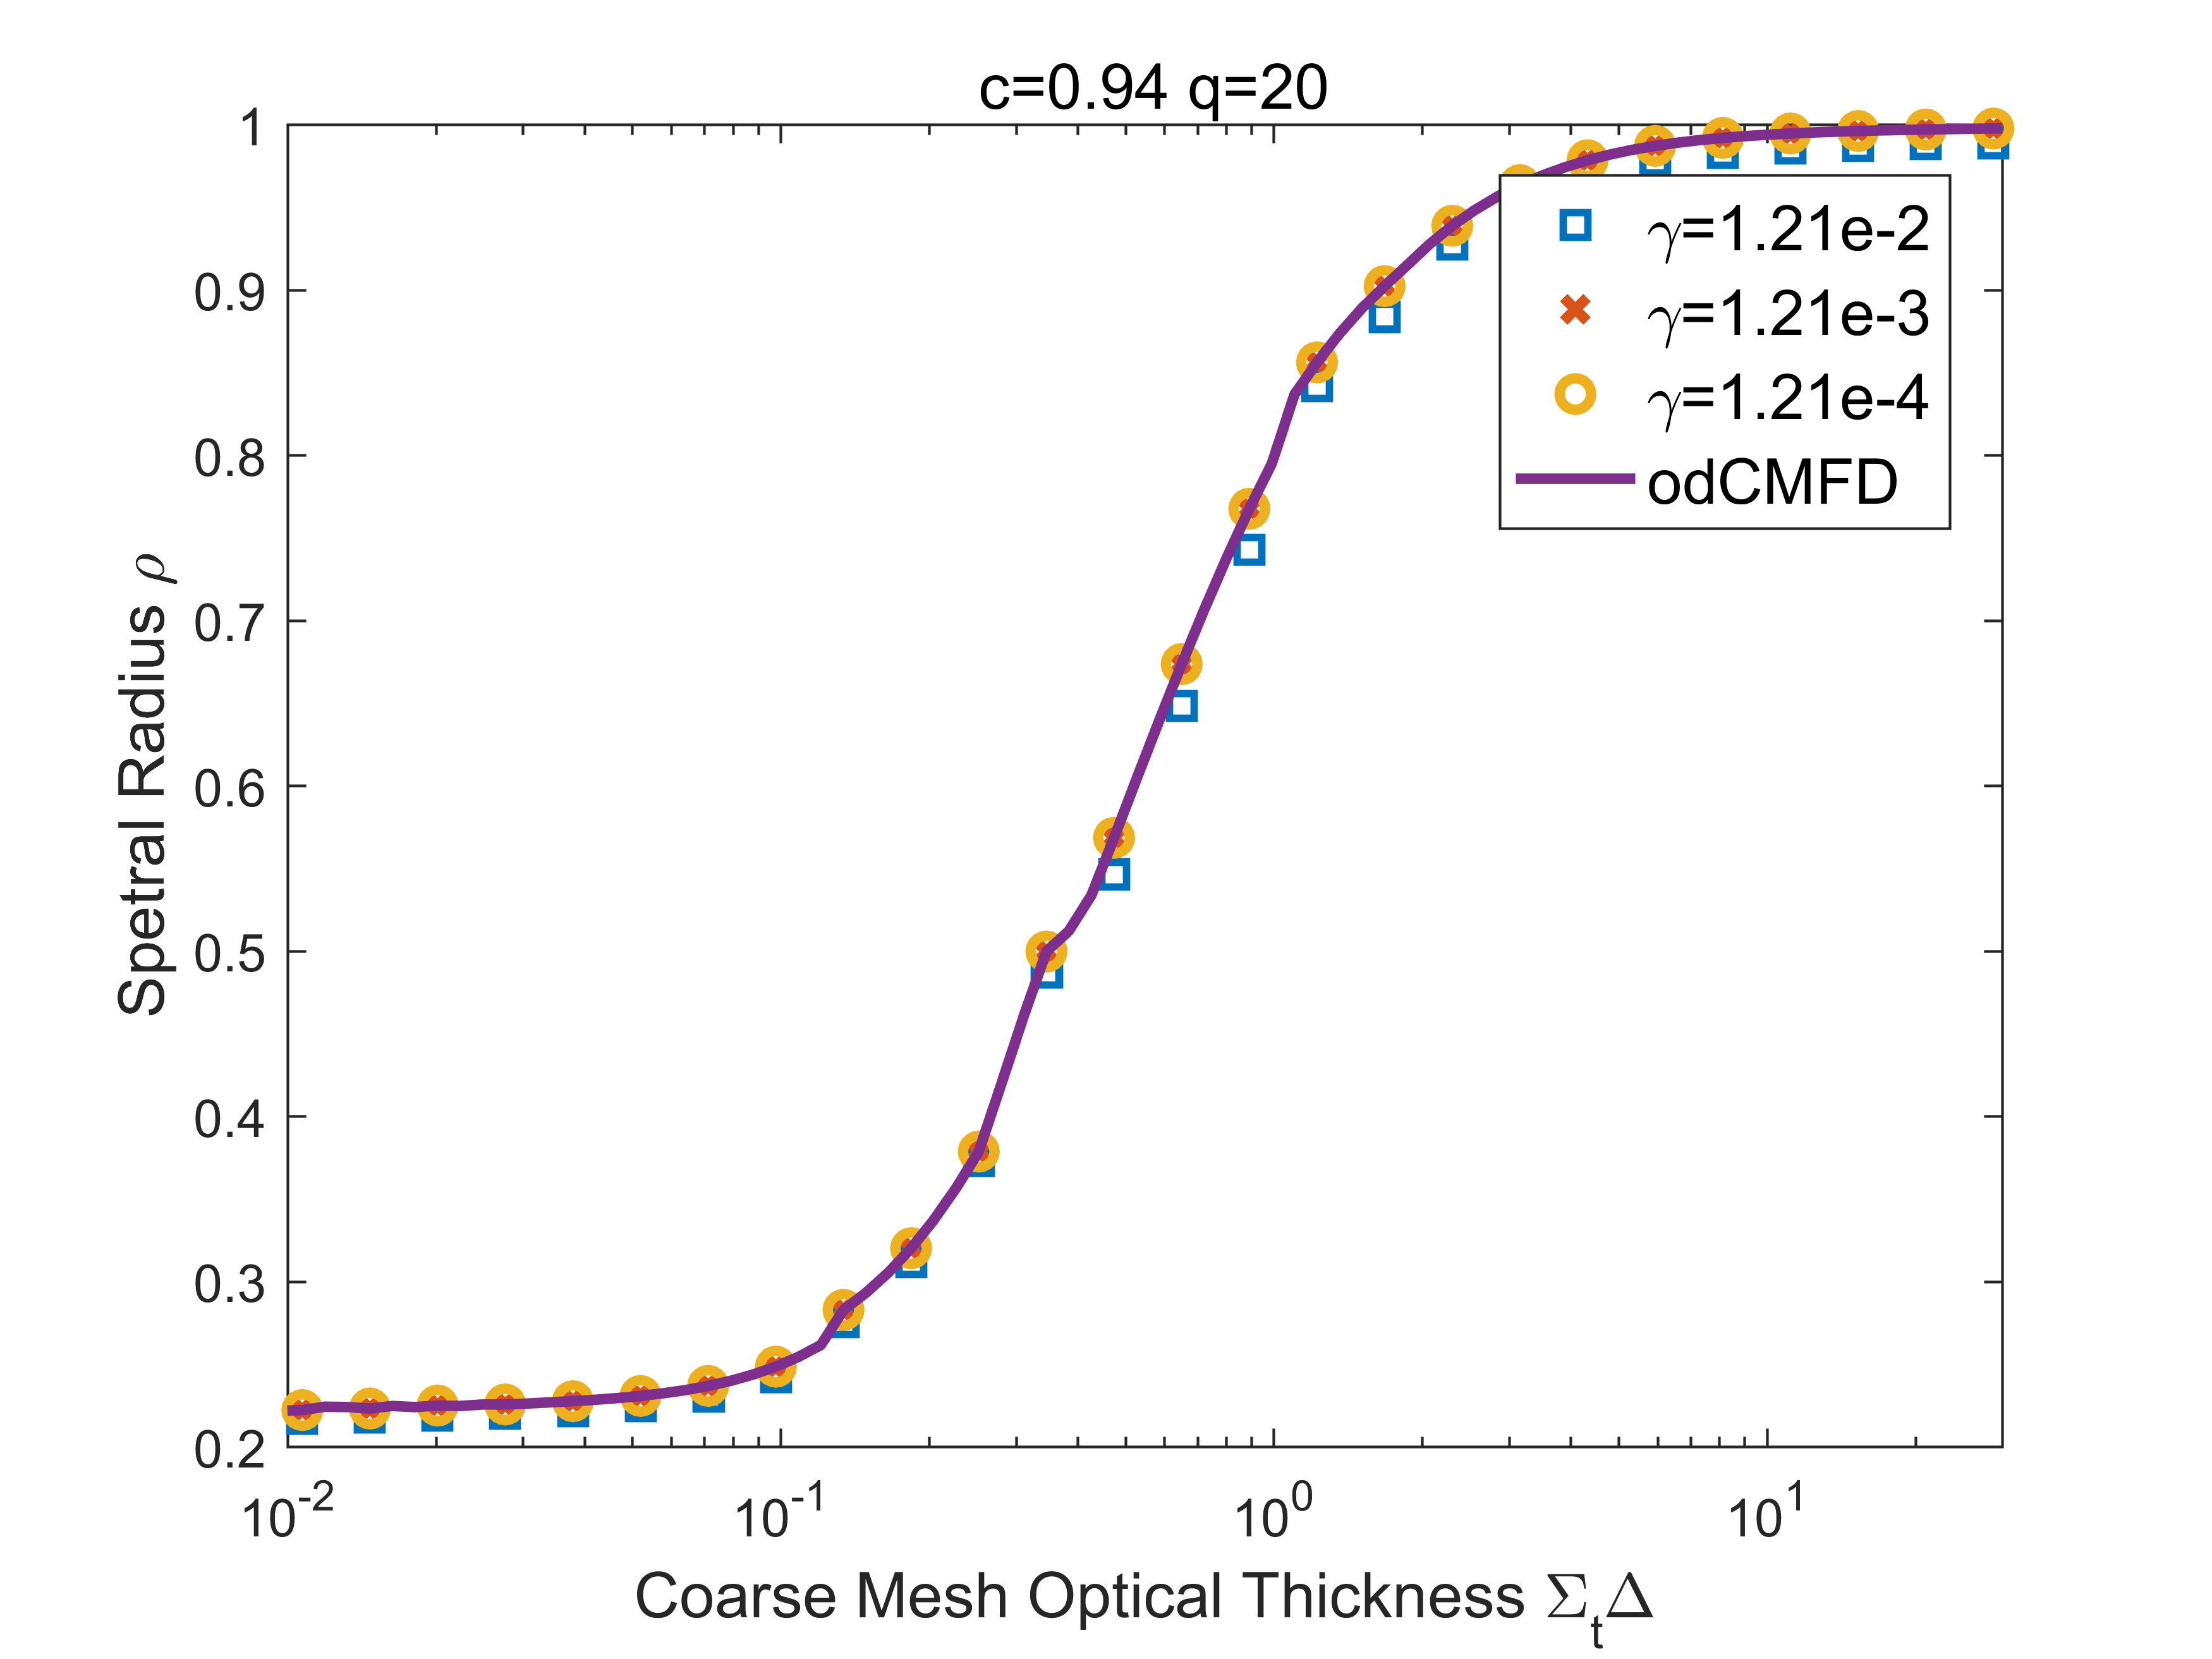
\includegraphics[width=\textwidth]{Texfile/Figure/CMFDoptimal.png}
	\end{subfigure}
\end{figure} 
\vspace{-1.5em}
\begin{itemize}
    \item $\omega=\frac{\pi}{200}$ is suggested.
    \item The same convergence behavior as NDA(CMFD) can be achieved theoretically.
\end{itemize}
\end{frame}
%%%%%%%%%%%%%%%%%%%%%%%%%%%%%%%%%%%%%%%%%%%%%%%%%%%%%%%%%%%%%%%%%%%%%%%%%%%%%%
\begin{frame}{Discussion of Near-optimal Partial Convergence}
\vspace{-1em}
 \begin{itemize}
     \item Pros:
     \begin{itemize}
         \item Easily to be implemented. Compatible with the CMFD and mutlilevel method such as MSED and Multilevel CMFD.
         \item Stablize the scheme and reduce the computational intensity.
     \end{itemize}
     \item Cons:
     \begin{itemize}
         \item $\gamma$ term needed to be calculated
         \item Derivation is based on $NDA$, may not be optimal for CMFD.
     \end{itemize}
     \item Conclusion: Intermediate solution to stabilize the Picard scheme with better efficiency. 
 \end{itemize}
 \end{frame}


\section{Conclusions}

%%%%%%%%%%%%%%%%%%%%%%%%%%%%%%%%%%%%%%%%%%%%%%%%%%%%%%%%%%%%%%%%%%%%%%%%%%%%%%%%%%%%%%%%%%%%%%%
\begin{frame}{Conclusions }
\begin{enumerate}
    \item The Fourier analysis of the iteration scheme accelerated by partially convergent NDA is performed. 
    \item The results support the observations that partial convergence can help to stabilize the multiphysics simulations, and near-optimal partial convergence exists though it is problem dependent.

    \item The partial convergence is shown to be equivalent to more well understood relaxation factor, and the relaxation factor induced by partially converging the lower-order problem is mainly imposed on the flat Fourier modes.

    \item The formula to determine the near-optimal partial convergence is put forward, provide people with intermediate measure to mitigate the stability issuse confronted in multiphysics simulation. 
\end{enumerate}
\end{frame}

%%%%%%%%%%%%%%%%%%%%%%%%%%%%%%%%%%%%%%%%%%%%%%%%%%%%%%%%%%%%%%%%%%%%%%%%%%%%%%%%%%%%%%%%%%%%%%%%%%%%%%%%%%%%%%%%%%%%%%%%%%%%%%%%%
%%%%%%%%%%%%%%%%%%%%%%%%%%%%%%%%%%%%%%%%%%%%%%%%%%%%%%%%%%%%%%%%%%%%%%%%%%%%%%%%%%%%%%%%%%%%%%%%%%%%%%%%%%%%%%%%%%%%%%%%%%%%%%%%%
\begin{frame}{Mext Step}
\begin{enumerate}
    \item Test the prediction from the Fourier analysis in realistic problem.
    \vspace{2em}
    \item Modify the iteration scheme in VERA-CS by using near-optimal partial convergence.
    \vspace{2em}
\end{enumerate}
 \end{frame}
%%%%%%%%%%%%%%%%%%


\section{Acknowledgement}
\begin{frame}
    \frametitle{Acknowledgments}
\begin{center}
 This research was supported by the Consortium for Advanced Simulation of Light Water Reactors (\url{www.casl.gov}), an Energy Innovation Hub (\url{http://www.energy.gov/hubs}) for Modeling and Simulation of Nuclear Reactors under U.S. Department of Energy Contract No. DE-AC05-00OR22725.
\end{center}
\vfill
\end{frame}

\begin{frame}{Afterwords}
\begin{enumerate}
    \item A lot of multilevel methods are being implemented. However, be cautious about using more power iterations or more aggressive Wielandt shift in feedback problems, especially on the coarsest space/energy grid.
    \item Be comfortable with a partially convergent NDA (CMFD). If it helps, just use it.
    \item A batch of MC particle simulation/deterministic source iteration is a power iteration, pencil-paper results suggest that we should avoid running a lot batches/source iterations in MC/deterministic codes before applying feedback.
\end{enumerate}
\end{frame}
\end{document}
